\documentclass[12pt,a4paper]{article}

\usepackage{fontspec}
\usepackage{polyglossia}
\setdefaultlanguage{greek}
\setotherlanguage{english}

\setmainfont[Script=Greek]{DejaVu Serif}
\setsansfont[Script=Greek]{DejaVu Sans}
\setmonofont[Script=Greek]{DejaVu Sans Mono}
\newfontfamily\greekfonttt[Script=Greek]{DejaVu Sans Mono}

\usepackage{geometry}
\usepackage{graphicx}
\usepackage{float}
\usepackage{caption}
\usepackage{subcaption}
\usepackage{xcolor}
\usepackage{listings}
\usepackage{amsmath}
\usepackage{amssymb}
\usepackage{booktabs}
\usepackage{longtable}
\usepackage{multirow}
\usepackage{array}
\usepackage[hidelinks]{hyperref}
\usepackage{fancyhdr}
\usepackage{tikz}
\usepackage{enumitem}
\usetikzlibrary{arrows.meta, shapes.geometric, positioning}

\geometry{left=2.5cm,right=2.5cm,top=2.5cm,bottom=2.5cm}

\definecolor{codegreen}{rgb}{0,0.6,0}
\definecolor{codegray}{rgb}{0.5,0.5,0.5}
\definecolor{backcolour}{rgb}{0.95,0.95,0.92}
\definecolor{theoremblue}{rgb}{0.85,0.90,1.0}
\definecolor{examplegreen}{rgb}{0.85,1.0,0.85}
\definecolor{warningyellow}{rgb}{1.0,0.97,0.80}
\definecolor{importantred}{rgb}{1.0,0.90,0.90}

\lstset{
    backgroundcolor=\color{backcolour},
    commentstyle=\color{codegreen},
    keywordstyle=\color{blue},
    basicstyle=\ttfamily\small,
    breaklines=true,
    numbers=left,
    numberstyle=\tiny\color{codegray},
    language=Python,
    frame=single
}

% Custom environments for educational boxes
\usepackage{tcolorbox}
\tcbuselibrary{skins, breakable}

\newtcolorbox{theorybox}[1][]{
    colback=theoremblue,
    colframe=blue!50!black,
    fonttitle=\bfseries,
    title=#1,
    breakable
}

\newtcolorbox{examplebox}[1][]{
    colback=examplegreen,
    colframe=green!50!black,
    fonttitle=\bfseries,
    title=#1,
    breakable
}

\newtcolorbox{warningbox}[1][]{
    colback=warningyellow,
    colframe=orange!60!black,
    fonttitle=\bfseries,
    title=#1,
    breakable
}

\newtcolorbox{importantbox}[1][]{
    colback=importantred,
    colframe=red!60!black,
    fonttitle=\bfseries,
    title=#1,
    breakable
}

\pagestyle{fancy}
\fancyhf{}
\rhead{AEM: 6931 -- Ρακοβαλής Παύλος}
\lhead{Ανάλυση Δεδομένων 2025-26}
\cfoot{\thepage}

\title{
    \textbf{Ανάλυση Δεδομένων 2025-26}\\[0.3cm]
    \Large 2η Εργασία: Ανάλυση Παλινδρόμησης\\[0.2cm]
    \large Πρόβλεψη Ποιότητας Κρασιού\\[0.5cm]
    \normalsize AEM: 6931
}
\author{Ρακοβαλής Παύλος}
\date{\today}

\begin{document}

\maketitle
\thispagestyle{fancy}

\tableofcontents
\newpage

%==========================================================================
% ΕΙΣΑΓΩΓΗ
%==========================================================================
\section{Εισαγωγή}

\subsection{Σκοπός της εργασίας}

Η παρούσα εργασία αποτελεί τη 2η εργασία του μαθήματος \textbf{Ανάλυση Δεδομένων} και έχει ως στόχο τη διερεύνηση κατά πόσο οι φυσικοχημικές ιδιότητες του κρασιού μπορούν να χρησιμοποιηθούν για την πρόβλεψη και ερμηνεία της \textbf{βαθμολογίας ποιότητας} (quality). Χρησιμοποιούνται τα καθαρισμένα δεδομένα από την 1η εργασία (τυχαίο δείγμα βάσει ΑΕΜ 6931, 5.274 παρατηρήσεις).

\subsection{Τι είναι η ανάλυση παλινδρόμησης;}

\begin{theorybox}[Ορισμός: Ανάλυση Παλινδρόμησης]
Η \textbf{ανάλυση παλινδρόμησης} (regression analysis) είναι μια στατιστική μέθοδος που μας επιτρέπει να μελετήσουμε τη σχέση μεταξύ μιας \textbf{εξαρτημένης μεταβλητής} (ή μεταβλητή απόκρισης) και μιας ή περισσότερων \textbf{ανεξάρτητων μεταβλητών} (ή προβλεπτικών μεταβλητών).

Στην ουσία, προσπαθούμε να απαντήσουμε στο ερώτημα: \textit{<<Μπορούμε να προβλέψουμε/εξηγήσουμε την τιμή μιας μεταβλητής χρησιμοποιώντας τις τιμές άλλων μεταβλητών;>>}
\end{theorybox}

\begin{examplebox}[Παράδειγμα από την καθημερινότητα]
Φανταστείτε ότι θέλετε να προβλέψετε τον βαθμό ενός φοιτητή σε ένα μάθημα. Ποιοι παράγοντες θα μπορούσαν να τον επηρεάσουν;
\begin{itemize}
    \item Ώρες μελέτης (όσο περισσότερο μελετάει, τόσο υψηλότερος ο βαθμός)
    \item Παρακολούθηση μαθημάτων (θετική επίδραση)
    \item Ώρες ύπνου πριν τις εξετάσεις (θετική επίδραση)
\end{itemize}
Η παλινδρόμηση μας δίνει μια \textbf{μαθηματική εξίσωση} που ποσοτικοποιεί αυτές τις σχέσεις.
\end{examplebox}

\subsection{Τα δεδομένα μας}

Χρησιμοποιούμε τα καθαρισμένα δεδομένα κρασιού από την 1η εργασία:

\begin{itemize}
    \item \textbf{Μεταβλητή απόκρισης} ($Y$): \texttt{quality} -- η βαθμολογία ποιότητας του κρασιού (ακέραιες τιμές 3--9)
    \item \textbf{Προβλεπτικές μεταβλητές} ($X_1, X_2, \ldots, X_{11}$):
    \begin{enumerate}
        \item \texttt{fixed acidity} -- σταθερή οξύτητα
        \item \texttt{volatile acidity} -- πτητική οξύτητα
        \item \texttt{citric acid} -- κιτρικό οξύ
        \item \texttt{residual sugar} -- υπολειπόμενη ζάχαρη
        \item \texttt{chlorides} -- χλωριούχα
        \item \texttt{free sulfur dioxide} -- ελεύθερο διοξείδιο του θείου
        \item \texttt{total sulfur dioxide} -- ολικό διοξείδιο του θείου
        \item \texttt{density} -- πυκνότητα
        \item \texttt{pH} -- δείκτης οξύτητας
        \item \texttt{sulphates} -- θειικά
        \item \texttt{alcohol} -- αλκοόλ
    \end{enumerate}
    \item \textbf{Πλήθος παρατηρήσεων}: 5.274
\end{itemize}

\subsection{Δομή της αναφοράς}

Η αναφορά οργανώνεται ως εξής:
\begin{itemize}
    \item \textbf{Ενότητα 2}: Απλή γραμμική παλινδρόμηση -- εξετάζουμε κάθε μεταβλητή ξεχωριστά
    \item \textbf{Ενότητα 3}: Πολλαπλή γραμμική παλινδρόμηση -- χρησιμοποιούμε όλες τις μεταβλητές μαζί
    \item \textbf{Ενότητα 4}: Πρόσω επιλογή μεταβλητών -- βρίσκουμε το βέλτιστο μοντέλο
    \item \textbf{Ενότητα 5}: Πολυωνυμική παλινδρόμηση -- μη γραμμικές σχέσεις
    \item \textbf{Ενότητα 6}: Κριτική αξιολόγηση του μοντέλου
\end{itemize}

%==========================================================================
% ΥΠΟΕΡΩΤΗΜΑ 1: ΑΠΛΗ ΓΡΑΜΜΙΚΗ ΠΑΛΙΝΔΡΟΜΗΣΗ
%==========================================================================
\newpage
\section{Απλή Γραμμική Παλινδρόμηση (Υποερώτημα 1)}

\subsection{Θεωρητικό υπόβαθρο}

\subsubsection{Τι είναι η απλή γραμμική παλινδρόμηση;}

\begin{theorybox}[Ορισμός: Απλή Γραμμική Παλινδρόμηση]
Η \textbf{απλή γραμμική παλινδρόμηση} (Simple Linear Regression -- SLR) είναι η απλούστερη μορφή παλινδρόμησης. Μελετά τη σχέση μεταξύ \textbf{μίας} ανεξάρτητης μεταβλητής $X$ και μιας εξαρτημένης μεταβλητής $Y$ μέσω ενός \textbf{γραμμικού μοντέλου}:

\begin{equation}
Y = \beta_0 + \beta_1 X + \varepsilon
\end{equation}

όπου:
\begin{itemize}
    \item $Y$ = η μεταβλητή απόκρισης (αυτό που θέλουμε να προβλέψουμε)
    \item $X$ = η προβλεπτική μεταβλητή (αυτό που χρησιμοποιούμε για πρόβλεψη)
    \item $\beta_0$ = η \textbf{τεταγμένη επί την αρχή} (intercept) -- η τιμή του $Y$ όταν $X = 0$
    \item $\beta_1$ = η \textbf{κλίση} (slope) -- πόσο αλλάζει το $Y$ όταν το $X$ αυξάνεται κατά 1 μονάδα
    \item $\varepsilon$ = το \textbf{σφάλμα} (error) -- η τυχαία διακύμανση που δεν εξηγείται από το μοντέλο
\end{itemize}
\end{theorybox}

\begin{examplebox}[Γεωμετρική ερμηνεία]
Φανταστείτε ότι σχεδιάζετε τα σημεία ($X$, $Y$) σε ένα γράφημα. Η γραμμική παλινδρόμηση <<περνάει>> μια ευθεία γραμμή μέσα από αυτά τα σημεία, με τρόπο τέτοιο ώστε η γραμμή να βρίσκεται \textbf{όσο πιο κοντά γίνεται} σε όλα τα σημεία.

Η $\beta_0$ μας λέει πού <<ξεκινάει>> η γραμμή (στον κάθετο άξονα), και η $\beta_1$ μας λέει αν η γραμμή \textbf{ανεβαίνει} ($\beta_1 > 0$, θετική σχέση) ή \textbf{κατεβαίνει} ($\beta_1 < 0$, αρνητική σχέση).
\end{examplebox}

\subsubsection{Η μέθοδος ελαχίστων τετραγώνων (\begin{english}OLS\end{english})}

\begin{theorybox}[Πώς υπολογίζονται οι συντελεστές;]
Η μέθοδος \textbf{Ελαχίστων Τετραγώνων} (Ordinary Least Squares -- OLS) βρίσκει τις τιμές $\beta_0$ και $\beta_1$ που \textbf{ελαχιστοποιούν} το άθροισμα των τετραγώνων των σφαλμάτων:

\begin{equation}
\min_{\beta_0, \beta_1} \sum_{i=1}^{n} (Y_i - \beta_0 - \beta_1 X_i)^2
\end{equation}

Δηλαδή, βρίσκει τη γραμμή που κάνει τα <<λάθη>> (τις αποστάσεις μεταξύ πραγματικών και προβλεπόμενων τιμών) \textbf{όσο μικρότερα γίνεται}. Τα σφάλματα υψώνονται στο τετράγωνο για δύο λόγους:
\begin{enumerate}
    \item Ώστε τα θετικά και αρνητικά σφάλματα να μην αλληλοεξουδετερώνονται
    \item Ώστε τα μεγάλα σφάλματα να <<τιμωρούνται>> περισσότερο
\end{enumerate}
\end{theorybox}

\subsubsection{Ο συντελεστής προσδιορισμού $R^2$}

\begin{theorybox}[Ορισμός: Συντελεστής Προσδιορισμού $R^2$]
Ο $R^2$ (R-squared) μας λέει \textbf{τι ποσοστό} της μεταβλητότητας του $Y$ εξηγείται από το μοντέλο:

\begin{equation}
R^2 = 1 - \frac{SS_{res}}{SS_{tot}} = 1 - \frac{\sum_{i=1}^{n}(Y_i - \hat{Y}_i)^2}{\sum_{i=1}^{n}(Y_i - \bar{Y})^2}
\end{equation}

όπου:
\begin{itemize}
    \item $SS_{res}$ = Residual Sum of Squares (μεταβλητότητα που \textbf{δεν} εξηγείται)
    \item $SS_{tot}$ = Total Sum of Squares (συνολική μεταβλητότητα)
    \item $\hat{Y}_i$ = η προβλεπόμενη τιμή για την παρατήρηση $i$
    \item $\bar{Y}$ = ο μέσος όρος του $Y$
\end{itemize}

\textbf{Ερμηνεία}:
\begin{itemize}
    \item $R^2 = 0$: Το μοντέλο δεν εξηγεί τίποτα (τόσο καλό όσο να προβλέπαμε πάντα τον μέσο όρο)
    \item $R^2 = 1$: Το μοντέλο εξηγεί τα πάντα (τέλεια πρόβλεψη)
    \item $R^2 = 0.60$: Το μοντέλο εξηγεί το 60\% της μεταβλητότητας
\end{itemize}
\end{theorybox}

\subsubsection{Έλεγχος στατιστικής σημαντικότητας}

Μέχρι τώρα μάθαμε πώς να φτιάχνουμε ένα μοντέλο παλινδρόμησης και πώς να μετράμε πόσο καλά ταιριάζει στα δεδομένα ($R^2$). Αλλά υπάρχει ένα κρίσιμο ερώτημα που \textbf{δεν} έχουμε απαντήσει ακόμα:

\textbf{Αυτή η σχέση που βρήκαμε, είναι πραγματική ή απλά τυχαία;}

\begin{examplebox}[Αναλογία: Το νόμισμα και η τύχη]
Φανταστείτε ότι ρίχνετε ένα νόμισμα 10 φορές και πέφτει \textbf{7 φορές κορώνα}. Είναι το νόμισμα <<πειραγμένο>> ή απλά τυχαίνει;

\begin{itemize}
    \item Αν ρίξετε 10 φορές και πέσει 7 κορώνες, λέτε: <<Μπα, μπορεί να είναι τύχη>>
    \item Αν ρίξετε 1000 φορές και πέσει 700 κορώνες, λέτε: <<Σίγουρα κάτι παίζει!>>
\end{itemize}

Ακριβώς αυτό κάνει ο \textbf{έλεγχος στατιστικής σημαντικότητας}: μας βοηθά να αποφασίσουμε αν αυτό που βλέπουμε στα δεδομένα μας είναι \textbf{πραγματικό φαινόμενο} ή απλά \textbf{τυχαίο θόρυβο}.
\end{examplebox}

\paragraph{Βήμα 1: Ορίζουμε δύο αντίθετες υποθέσεις.}

Πριν κάνουμε τον έλεγχο, πρέπει να διατυπώσουμε ακριβώς τι θέλουμε να ελέγξουμε. Για κάθε μεταβλητή $X$ ορίζουμε δύο \textbf{υποθέσεις}:

\begin{theorybox}[Ορισμός: Μηδενική και Εναλλακτική Υπόθεση]
\begin{itemize}
    \item $H_0: \beta_1 = 0$ \quad \textbf{Μηδενική υπόθεση} (Null Hypothesis)

    Σημαίνει: <<Η μεταβλητή $X$ \textbf{δεν} επηρεάζει \textbf{καθόλου} το $Y$. Η κλίση της γραμμής είναι μηδέν, δηλαδή η γραμμή είναι εντελώς \textbf{οριζόντια}. Δεν υπάρχει καμία σχέση.>>

    \item $H_1: \beta_1 \neq 0$ \quad \textbf{Εναλλακτική υπόθεση} (Alternative Hypothesis)

    Σημαίνει: <<Η μεταβλητή $X$ \textbf{επηρεάζει} το $Y$. Η κλίση δεν είναι μηδέν -- η γραμμή ανεβαίνει ή κατεβαίνει, άρα υπάρχει σχέση.>>
\end{itemize}
\end{theorybox}

\begin{examplebox}[Αναλογία: Δικαστήριο -- <<Αθώος μέχρι αποδείξεως του εναντίου>>]
Ο έλεγχος υποθέσεων λειτουργεί ακριβώς σαν δικαστήριο:

\begin{enumerate}
    \item \textbf{Ξεκινάμε υποθέτοντας αθωότητα}: Η $H_0$ λέει <<δεν υπάρχει σχέση>> -- αυτή είναι η <<αθωότητα>>. Την θεωρούμε αληθή εξ αρχής.

    \item \textbf{Ψάχνουμε αποδείξεις}: Κοιτάμε τα δεδομένα μας. Αν τα δεδομένα δείχνουν ισχυρή σχέση, αυτό είναι <<απόδειξη>> κατά της αθωότητας.

    \item \textbf{Αποφασίζουμε}: Αν οι αποδείξεις είναι αρκετά ισχυρές (πέρα από κάθε λογική αμφιβολία), τότε <<καταδικάζουμε>> -- δηλαδή \textbf{απορρίπτουμε} την $H_0$ και λέμε ότι υπάρχει σχέση. Αν δεν είναι αρκετές, <<αθωώνουμε>> -- \textbf{δεν απορρίπτουμε} την $H_0$.
\end{enumerate}

\textbf{Σημαντικό}: Ακριβώς όπως στο δικαστήριο δεν λέμε ποτέ <<αποδείχθηκε η αθωότητα>> (απλά <<δεν αποδείχθηκε η ενοχή>>), έτσι και εδώ δεν λέμε ποτέ <<αποδείξαμε ότι δεν υπάρχει σχέση>>. Λέμε απλά <<δεν βρήκαμε αρκετές αποδείξεις για σχέση>>.
\end{examplebox}

\paragraph{Βήμα 2: Υπολογίζουμε την <<απόδειξη>> -- ο t-έλεγχος.}

Τώρα χρειαζόμαστε ένα \textbf{αριθμητικό μέτρο} για το πόσο ισχυρή είναι η <<απόδειξη>> κατά της $H_0$. Αυτό το μέτρο λέγεται \textbf{t-στατιστική} (t-statistic):

\begin{theorybox}[Ορισμός: Η t-στατιστική]
\begin{equation}
t = \frac{\hat{\beta}_1}{SE(\hat{\beta}_1)}
\end{equation}

Ας αναλύσουμε κάθε κομμάτι:
\begin{itemize}
    \item $\hat{\beta}_1$ = η \textbf{κλίση} που υπολόγισε το μοντέλο μας. Αυτή είναι η <<εκτίμησή>> μας για τη σχέση μεταξύ $X$ και $Y$.
    \item $SE(\hat{\beta}_1)$ = το \textbf{τυπικό σφάλμα} (Standard Error) της κλίσης. Αυτή είναι η <<αβεβαιότητα>> στην εκτίμησή μας -- πόσο θα μπορούσε να διαφέρει η $\hat{\beta}_1$ αν είχαμε πάρει \textbf{διαφορετικό} δείγμα κρασιών.
\end{itemize}

Με λόγια: η t-στατιστική μετράει \textbf{πόσες φορές μεγαλύτερη} είναι η κλίση που βρήκαμε σε σχέση με την αβεβαιότητα.
\end{theorybox}

\begin{examplebox}[Αναλογία: Σήμα εναντίον θορύβου στο ραδιόφωνο]
Φανταστείτε ότι ακούτε ραδιόφωνο στο αυτοκίνητο:

\begin{itemize}
    \item \textbf{Η κλίση $\hat{\beta}_1$ είναι η <<φωνή>>} (σήμα): Πόσο δυνατά ακούγεται ο εκφωνητής. Αν η κλίση είναι μεγάλη, η <<φωνή>> είναι δυνατή -- βλέπουμε ισχυρή σχέση.

    \item \textbf{Το τυπικό σφάλμα $SE$ είναι ο <<θόρυβος>>}: Πόση παρασιτική βοή υπάρχει. Αν το $SE$ είναι μεγάλο, σημαίνει ότι η εκτίμησή μας είναι αναξιόπιστη -- υπάρχει πολύς <<θόρυβος>>.

    \item \textbf{Η t-στατιστική είναι η αναλογία σήματος προς θόρυβο}: Πόσο καθαρά ακούτε τον εκφωνητή πάνω από τη βοή.
\end{itemize}

\textbf{Παράδειγμα}: Αν $\hat{\beta}_1 = 0.343$ και $SE = 0.00977$:
$$t = \frac{0.343}{0.00977} = 35.1$$

Αυτό σημαίνει: η κλίση είναι \textbf{35 φορές} μεγαλύτερη από την αβεβαιότητα! Ένα τεράστιο σήμα -- σαν να ακούτε εκφωνητή σε ένα ήσυχο δωμάτιο.

Αντίθετα, αν είχαμε $\hat{\beta}_1 = 0.01$ και $SE = 0.02$:
$$t = \frac{0.01}{0.02} = 0.5$$

Η κλίση είναι \textbf{μικρότερη} από την αβεβαιότητα! Ένα πολύ αδύναμο σήμα -- σαν να προσπαθείτε να ακούσετε κάποιον να ψιθυρίζει σε συναυλία ροκ.

\textbf{Κανόνας}: Όσο πιο μακριά είναι η $|t|$ από το μηδέν, τόσο πιο ισχυρή η <<απόδειξη>> ότι η σχέση είναι πραγματική.
\end{examplebox}

\begin{theorybox}[Τι είναι ακριβώς το Τυπικό Σφάλμα (Standard Error);]
Ας καταλάβουμε γιατί χρειαζόμαστε το $SE$:

Φανταστείτε ότι πηγαίνετε σε 100 διαφορετικά σούπερ μάρκετ και δοκιμάζετε κρασιά. Σε κάθε σούπερ μάρκετ θα βρείτε \textbf{λίγο διαφορετική} σχέση μεταξύ αλκοόλ και ποιότητας, γιατί σε κάθε κατάστημα υπάρχουν \textbf{διαφορετικά} κρασιά.

\begin{itemize}
    \item Ένα σούπερ μάρκετ μπορεί να δώσει $\hat{\beta}_1 = 0.32$
    \item Ένα άλλο $\hat{\beta}_1 = 0.36$
    \item Ένα τρίτο $\hat{\beta}_1 = 0.34$
\end{itemize}

Αν \textbf{τα περισσότερα σούπερ μάρκετ} δίνουν παρόμοια αποτελέσματα (π.χ. 0.32--0.36), τότε η εκτίμησή μας είναι \textbf{σταθερή} και αξιόπιστη $\Rightarrow$ \textbf{μικρό} $SE$.

Αν τα αποτελέσματα κυμαίνονται ευρέως (π.χ. $-0.10$ ως $+0.80$), τότε δεν μπορούμε να εμπιστευτούμε κανένα μεμονωμένο αποτέλεσμα $\Rightarrow$ \textbf{μεγάλο} $SE$.

Το $SE$ μας λέει πόσο \textbf{θα <<κουνιόταν>>} η εκτίμησή μας αν επαναλαμβάναμε το πείραμα πολλές φορές.
\end{theorybox}

\paragraph{Βήμα 3: Μετατρέπουμε το $t$ σε πιθανότητα -- η p-value.}

Η t-στατιστική μας λέει πόσο ισχυρό είναι το σήμα, αλλά χρειαζόμαστε κάτι πιο κατανοητό: μια \textbf{πιθανότητα}. Εδώ μπαίνει η p-value.

\begin{theorybox}[Ορισμός: Η p-value -- Βήμα προς βήμα]
Η \textbf{p-value} απαντάει στο εξής ερώτημα:

\begin{center}
\fbox{\parbox{0.85\textwidth}{\centering
<<Αν η $H_0$ ήταν αληθής (δηλαδή αν πραγματικά \textbf{δεν} υπήρχε καμία σχέση μεταξύ $X$ και $Y$), ποια θα ήταν η πιθανότητα να παρατηρούσαμε t-στατιστική τόσο ακραία ή πιο ακραία από αυτή που βρήκαμε;>>
}}
\end{center}

\textbf{Με πιο απλά λόγια}: <<Πόσο πιθανό είναι η τύχη να <<μιμηθεί>> μια τόσο ισχυρή σχέση;>>
\end{theorybox}

\begin{examplebox}[Αναλογία: Ρίψεις νομίσματος -- Κατανόηση της p-value]
Ας γυρίσουμε στο παράδειγμα με το νόμισμα:

\textbf{Σενάριο}: Ένας φίλος σας λέει ότι το νόμισμά του είναι δίκαιο ($H_0$: πιθανότητα κορώνας = 50\%). Εσείς θέλετε να ελέγξετε αν λέει αλήθεια.

\textbf{Πείραμα 1}: Ρίχνετε 10 φορές, πέφτουν 7 κορώνες.
\begin{itemize}
    \item Ρωτάτε: <<Αν το νόμισμα ΕΙΝΑΙ δίκαιο, πόσο πιθανό είναι να πέσουν 7+ κορώνες στις 10;>>
    \item Η απάντηση (η p-value): περίπου 17\%
    \item Ερμηνεία: <<Ε, ένα δίκαιο νόμισμα θα έδινε 7+ κορώνες περίπου 1 στις 6 φορές. Δεν είναι τόσο ασυνήθιστο. Πιθανόν απλά τύχη.>>
    \item \textbf{Δεν απορρίπτουμε} την $H_0$. Δεν μπορούμε να πούμε ότι το νόμισμα είναι πειραγμένο.
\end{itemize}

\textbf{Πείραμα 2}: Ρίχνετε 1000 φορές, πέφτουν 700 κορώνες.
\begin{itemize}
    \item Ρωτάτε: <<Αν το νόμισμα ΕΙΝΑΙ δίκαιο, πόσο πιθανό είναι να πέσουν 700+ κορώνες στις 1000;>>
    \item Η απάντηση (η p-value): πρακτικά 0\% (κάτι σαν $10^{-50}$)
    \item Ερμηνεία: <<Θα ήταν σχεδόν αδύνατο ένα δίκαιο νόμισμα να δώσει 700 κορώνες στις 1000. Κάτι άλλο συμβαίνει.>>
    \item \textbf{Απορρίπτουμε} την $H_0$. Το νόμισμα σχεδόν σίγουρα δεν είναι δίκαιο.
\end{itemize}

\textbf{Στην παλινδρόμηση}: Αντί για νομίσματα, ρωτάμε: <<Αν ΠΡΑΓΜΑΤΙΚΑ δεν υπήρχε σχέση μεταξύ αλκοόλ και ποιότητας, πόσο πιθανό θα ήταν να βρούμε $t = 35.1$;>>. Η p-value $= 4.55 \times 10^{-243}$ -- ένας αριθμός τόσο κοντά στο μηδέν που είναι \textbf{αδιανόητο} να πρόκειται για τύχη.
\end{examplebox}

\paragraph{Βήμα 4: Αποφασίζουμε -- το κατώφλι $\alpha = 0.05$.}

\begin{theorybox}[Ορισμός: Το επίπεδο σημαντικότητας $\alpha$]
Πριν κάνουμε τον έλεγχο, ορίζουμε ένα \textbf{κατώφλι}: πόσο μικρή πρέπει να είναι η p-value για να μας πείσει. Αυτό το κατώφλι λέγεται \textbf{επίπεδο σημαντικότητας} (significance level) και συμβολίζεται $\alpha$.

\textbf{Η σύμβαση}: Στις περισσότερες επιστήμες χρησιμοποιούμε $\alpha = 0.05$ (5\%). Αυτό σημαίνει:

<<Αν η πιθανότητα να βλέπουμε τέτοιο αποτέλεσμα τυχαία είναι μικρότερη από 5\%, τότε λέμε ότι η σχέση είναι \textbf{στατιστικά σημαντική}.>>

\textbf{Ο κανόνας απόφασης}:
\begin{itemize}
    \item Αν p-value $< \alpha = 0.05$ $\Rightarrow$ \textbf{Απορρίπτουμε} την $H_0$ $\Rightarrow$ Η σχέση \textbf{είναι} στατιστικά σημαντική
    \item Αν p-value $\geq \alpha = 0.05$ $\Rightarrow$ \textbf{Δεν απορρίπτουμε} την $H_0$ $\Rightarrow$ \textbf{Δεν μπορούμε} να πούμε ότι υπάρχει σχέση
\end{itemize}
\end{theorybox}

\begin{examplebox}[title={Γιατί ακριβώς $\alpha = 0.05$ και όχι κάτι άλλο;}]
Η τιμή 0.05 (5\%) είναι μια \textbf{σύμβαση}, όχι φυσικός νόμος. Επιλέχθηκε ιστορικά (από τον Ronald Fisher, τη δεκαετία του 1920) ως ένα λογικό ισοζύγιο:

\begin{itemize}
    \item Πολύ αυστηρό κατώφλι (π.χ. $\alpha = 0.001$): Θα χάναμε πολλές αληθινές σχέσεις (θα λέγαμε <<δεν υπάρχει σχέση>> ενώ υπάρχει)
    \item Πολύ χαλαρό κατώφλι (π.χ. $\alpha = 0.20$): Θα <<βρίσκαμε>> σχέσεις που δεν υπάρχουν (θα πέφταμε θύματα της τύχης)
    \item Το 5\% θεωρείται αποδεκτός συμβιβασμός: <<Δέχομαι 5\% πιθανότητα να κάνω λάθος>>
\end{itemize}

Σε ορισμένα πεδία χρησιμοποιούνται αυστηρότερα κατώφλια. Π.χ. στη φυσική σωματιδίων, η ανακάλυψη του Higgs boson απαιτούσε $\alpha = 0.0000003$ (<<5 sigma>>)!
\end{examplebox}

\paragraph{Ας δούμε ολόκληρη τη διαδικασία με ένα πραγματικό παράδειγμα.}

\begin{examplebox}[Πλήρες παράδειγμα: Αλκοόλ $\to$ Ποιότητα]
\textbf{Ερώτηση}: <<Επηρεάζει το αλκοόλ την ποιότητα του κρασιού, ή είναι τυχαίο;>>

\textbf{Βήμα 1 -- Υποθέσεις}:
\begin{itemize}
    \item $H_0$: Το αλκοόλ \textbf{δεν} επηρεάζει την ποιότητα ($\beta_1 = 0$)
    \item $H_1$: Το αλκοόλ \textbf{επηρεάζει} την ποιότητα ($\beta_1 \neq 0$)
\end{itemize}

\textbf{Βήμα 2 -- Υπολογισμός}:
\begin{itemize}
    \item Από τα δεδομένα μας βρίσκουμε: $\hat{\beta}_1 = 0.3430$ (η κλίση)
    \item Η αβεβαιότητα αυτής της εκτίμησης: $SE = 0.00977$
    \item Η t-στατιστική: $t = \frac{0.3430}{0.00977} = 35.13$
    \item Η κλίση είναι \textbf{35 φορές} μεγαλύτερη από την αβεβαιότητα!
\end{itemize}

\textbf{Βήμα 3 -- p-value}:
\begin{itemize}
    \item Ρωτάμε: <<Αν δεν υπήρχε ΚΑΜΙΑ σχέση, πόσο πιθανό θα ήταν να βρούμε $t = 35.13$;>>
    \item Απάντηση: $p = 4.55 \times 10^{-243}$
    \item Αυτός ο αριθμός είναι ένα 0 ακολουθούμενο από 242 μηδενικά και μετά ένα 455. Για αναφορά, τα άτομα στο σύμπαν είναι περίπου $10^{80}$ -- αυτή η p-value είναι ασύλληπτα μικρή.
\end{itemize}

\textbf{Βήμα 4 -- Απόφαση}:
\begin{itemize}
    \item $4.55 \times 10^{-243} < 0.05$; \textbf{ΝΑΙ}, κατά πολύ!
    \item \textbf{Απορρίπτουμε} την $H_0$
    \item \textbf{Συμπέρασμα}: Η σχέση μεταξύ αλκοόλ και ποιότητας είναι \textbf{στατιστικά σημαντική}. Δεν πρόκειται για τύχη.
\end{itemize}
\end{examplebox}

\begin{warningbox}[title={Τρεις συχνές παρανοήσεις για τη p-value}]
Η p-value είναι ίσως η πιο \textbf{παρεξηγημένη} έννοια στη στατιστική. Ας ξεκαθαρίσουμε τρία λάθη:

\textbf{Παρανόηση 1}: <<Η p-value μας λέει πόσο ισχυρή είναι η σχέση.>>
\begin{itemize}
    \item \textbf{ΛΑΘΟΣ}! Η p-value μας λέει μόνο αν η σχέση είναι \textbf{στατιστικά σημαντική} (δηλαδή, αν δεν οφείλεται σε τύχη), ΟΧΙ πόσο ισχυρή είναι.
    \item Παράδειγμα: Με πολλά δεδομένα (π.χ. 5.320 κρασιά), ακόμα και μια \textbf{πολύ αδύναμη} σχέση μπορεί να δώσει πολύ μικρή p-value.
    \item Το pH έχει p-value = 0.028 (στατιστικά σημαντική) αλλά $R^2 = 0.0009$ -- εξηγεί μόλις 0.09\% της μεταβλητότητας!
    \item \textbf{Για την ισχύ κοιτάμε τον $R^2$, όχι τη p-value}.
\end{itemize}

\textbf{Παρανόηση 2}: <<Αν η p-value $> 0.05$, σημαίνει ότι δεν υπάρχει σχέση.>>
\begin{itemize}
    \item \textbf{ΛΑΘΟΣ}! Σημαίνει μόνο ότι \textbf{δεν βρήκαμε αρκετές αποδείξεις} για να πούμε ότι υπάρχει σχέση. Ίσως υπάρχει αλλά δεν είχαμε αρκετά δεδομένα, ή ίσως η σχέση δεν είναι γραμμική.
    \item Η <<απουσία απόδειξης>> δεν είναι <<απόδειξη απουσίας>>.
\end{itemize}

\textbf{Παρανόηση 3}: <<Η p-value = 0.03 σημαίνει ότι υπάρχει 3\% πιθανότητα η $H_0$ να είναι αληθής.>>
\begin{itemize}
    \item \textbf{ΛΑΘΟΣ}! Η p-value δεν μας λέει την πιθανότητα της $H_0$. Μας λέει: <<αν η $H_0$ ΗΤΑΝ αληθής, πόσο πιθανά θα ήταν τα δεδομένα μας;>> -- αυτό είναι \textbf{τελείως διαφορετικό} ερώτημα.
    \item Αναλογία: Αν βρέχει, η πιθανότητα ο δρόμος να είναι βρεγμένος είναι 100\%. Αλλά αν ο δρόμος είναι βρεγμένος, δεν σημαίνει 100\% ότι βρέχει (μπορεί να πέρασε βυτιοφόρο)!
\end{itemize}
\end{warningbox}

\begin{importantbox}[Σύνοψη: Πώς λειτουργεί ο έλεγχος σε 4 βήματα]
\begin{enumerate}
    \item \textbf{Υποθέτουμε} ότι δεν υπάρχει σχέση ($H_0: \beta_1 = 0$)
    \item \textbf{Μετράμε} πόσο ισχυρή είναι η σχέση σε σύγκριση με τον θόρυβο (t-στατιστική $= \frac{\text{σήμα}}{\text{θόρυβος}}$)
    \item \textbf{Υπολογίζουμε} πόσο πιθανό θα ήταν να βλέπαμε τέτοιο σήμα αν δεν υπήρχε σχέση (p-value)
    \item \textbf{Αποφασίζουμε}: αν η p-value $< 0.05$, η σχέση είναι πραγματική. Αν η p-value $\geq 0.05$, δεν μπορούμε να αποφανθούμε.
\end{enumerate}
\end{importantbox}

\subsection{Αποτελέσματα: Μοντέλα απλής γραμμικής παλινδρόμησης}

Για κάθε μία από τις 11 προβλεπτικές μεταβλητές, εφαρμόστηκε ένα μοντέλο της μορφής:
$$\text{quality} = \beta_0 + \beta_1 \cdot X_j + \varepsilon$$

Τα αποτελέσματα παρουσιάζονται στον Πίνακα~\ref{tab:simple_regression}, ταξινομημένα κατά φθίνουσα σειρά $R^2$ (δηλαδή, πρώτα η μεταβλητή που εξηγεί τη μεγαλύτερη μεταβλητότητα).

\begin{table}[H]
\centering
\caption{Αποτελέσματα Απλής Γραμμικής Παλινδρόμησης: quality $\sim$ κάθε μεταβλητή}
\label{tab:simple_regression}
\small
\begin{tabular}{lccccc}
\toprule
\textbf{Μεταβλητή} & $\hat{\beta}_1$ & \textbf{t-stat} & \textbf{p-value} & $R^2$ & \textbf{Σημαντ.} \\
\midrule
\begin{english}alcohol\end{english} & 0.3430 & 35.13 & $4.55 \times 10^{-243}$ & 0.1897 & Ναι \\
\begin{english}density\end{english} & $-94.21$ & $-23.40$ & $2.64 \times 10^{-115}$ & 0.0941 & Ναι \\
\begin{english}volatile acidity\end{english} & $-1.386$ & $-19.08$ & $1.59 \times 10^{-78}$ & 0.0646 & Ναι \\
\begin{english}chlorides\end{english} & $-5.078$ & $-15.09$ & $2.17 \times 10^{-50}$ & 0.0414 & Ναι \\
\begin{english}citric acid\end{english} & 0.5662 & 6.86 & $7.54 \times 10^{-12}$ & 0.0089 & Ναι \\
\begin{english}fixed acidity\end{english} & $-0.0516$ & $-5.24$ & $1.68 \times 10^{-7}$ & 0.0052 & Ναι \\
\begin{english}residual sugar\end{english} & $-0.0101$ & $-3.88$ & $1.04 \times 10^{-4}$ & 0.0029 & Ναι \\
\begin{english}total sulfur dioxide\end{english} & $-0.0008$ & $-3.79$ & $1.50 \times 10^{-4}$ & 0.0027 & Ναι \\
\begin{english}free sulfur dioxide\end{english} & 0.0026 & 3.79 & $1.55 \times 10^{-4}$ & 0.0027 & Ναι \\
\begin{english}sulphates\end{english} & 0.2528 & 3.09 & $2.02 \times 10^{-3}$ & 0.0018 & Ναι \\
\begin{english}pH\end{english} & 0.1745 & 2.19 & $2.84 \times 10^{-2}$ & 0.0009 & Ναι \\
\bottomrule
\end{tabular}
\end{table}

\subsubsection{Ερμηνεία αποτελεσμάτων}

\textbf{Βασικά ευρήματα:}

\begin{enumerate}
    \item \textbf{Όλες} οι 11 μεταβλητές έχουν \textbf{στατιστικά σημαντική} σχέση με την ποιότητα ($p < 0.05$).

    \item Ωστόσο, η \textbf{ισχύς} αυτής της σχέσης ποικίλλει δραματικά:
    \begin{itemize}
        \item Το \textbf{αλκοόλ} (alcohol) είναι μακράν ο ισχυρότερος μεμονωμένος προβλέπτης ($R^2 = 0.19$), εξηγώντας σχεδόν 19\% της μεταβλητότητας. Κάθε αύξηση κατά 1 βαθμό αλκοόλ αντιστοιχεί σε αύξηση βαθμολογίας κατά 0.34 μονάδες.
        \item Η \textbf{πυκνότητα} (density) ακολουθεί ($R^2 = 0.094$) με αρνητική σχέση -- τα πιο πυκνά κρασιά τείνουν να βαθμολογούνται χαμηλότερα.
        \item Η \textbf{πτητική οξύτητα} (volatile acidity) έχει $R^2 = 0.065$ με ισχυρά αρνητική σχέση -- μεγαλύτερη πτητική οξύτητα σημαίνει χαμηλότερη ποιότητα (η πτητική οξύτητα συνδέεται με δυσάρεστη ξινή γεύση).
        \item Οι υπόλοιπες μεταβλητές έχουν πολύ χαμηλό $R^2$ ($< 0.05$), υποδεικνύοντας ασθενείς μεμονωμένες σχέσεις.
    \end{itemize}

    \item \textbf{Κατεύθυνση σχέσεων}:
    \begin{itemize}
        \item \textbf{Θετική} (υψηλότερες τιμές $\Rightarrow$ υψηλότερη ποιότητα): alcohol, citric acid, free sulfur dioxide, sulphates, pH
        \item \textbf{Αρνητική} (υψηλότερες τιμές $\Rightarrow$ χαμηλότερη ποιότητα): density, volatile acidity, chlorides, fixed acidity, residual sugar, total sulfur dioxide
    \end{itemize}
\end{enumerate}

\begin{importantbox}[Γιατί τα $R^2$ είναι τόσο χαμηλά;]
Ακόμα και η καλύτερη μεταβλητή (alcohol) εξηγεί μόνο 19\% της μεταβλητότητας. Αυτό σημαίνει ότι η ποιότητα του κρασιού είναι ένα \textbf{πολυπαράγοντικό} φαινόμενο -- καμία μεμονωμένη μεταβλητή δεν αρκεί για να την εξηγήσει. Γι' αυτό χρειαζόμαστε την \textbf{πολλαπλή} παλινδρόμηση (Ενότητα 3).
\end{importantbox}

\subsection{Διαγράμματα διασποράς}

Στο Σχήμα~\ref{fig:scatter} παρουσιάζονται τα διαγράμματα διασποράς για τις στατιστικά σημαντικές μεταβλητές, μαζί με τη γραμμή παλινδρόμησης.

\begin{figure}[H]
    \centering
    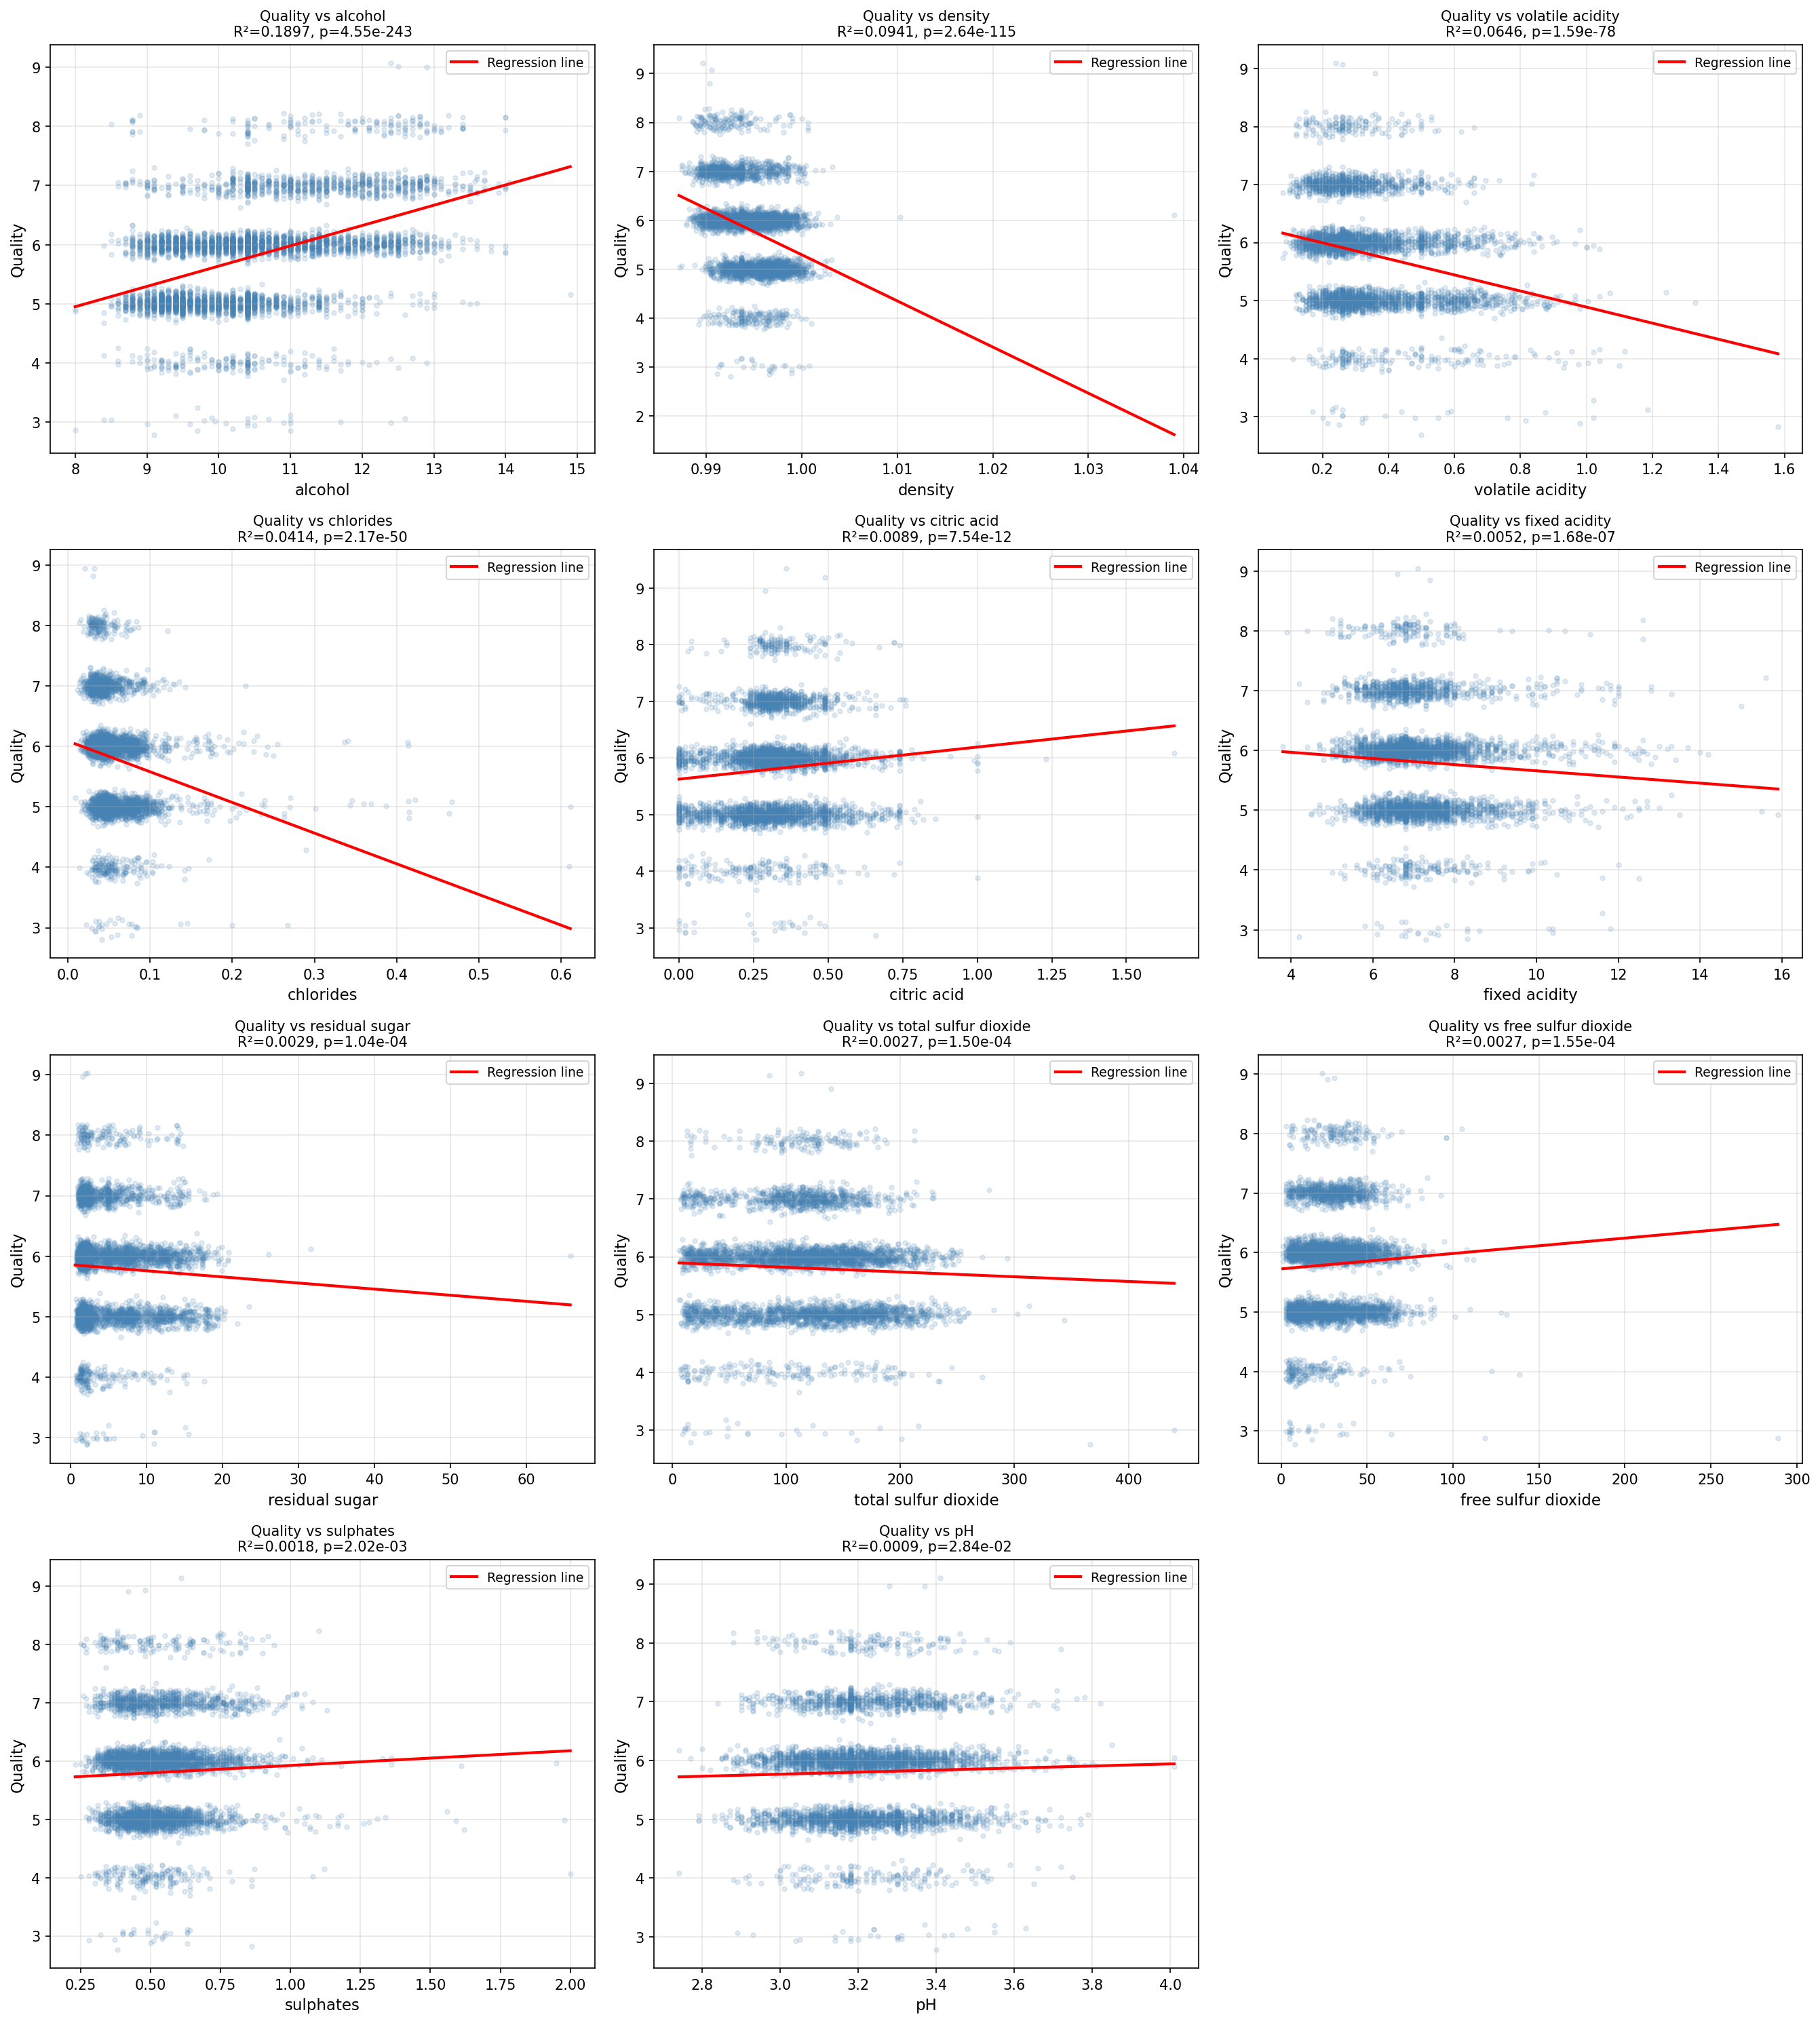
\includegraphics[width=\textwidth]{scatter_plots_significant.png}
    \caption{Διαγράμματα διασποράς μεταξύ ποιότητας και κάθε μεταβλητής. Η κόκκινη γραμμή αντιπροσωπεύει τη γραμμή παλινδρόμησης. Ένα μικρό τυχαίο jitter έχει προστεθεί στη μεταβλητή quality για καλύτερη οπτικοποίηση (η quality παίρνει ακέραιες τιμές).}
    \label{fig:scatter}
\end{figure}

\begin{theorybox}[Τι είναι το διάγραμμα διασποράς;]
Ένα \textbf{διάγραμμα διασποράς} (scatter plot) είναι ένα γράφημα όπου κάθε \textbf{σημείο} αντιπροσωπεύει μία παρατήρηση. Η θέση του σημείου καθορίζεται από τις τιμές δύο μεταβλητών (μία σε κάθε άξονα).

Αν τα σημεία σχηματίζουν ένα \textbf{ανοδικό νέφος}, η σχέση είναι θετική. Αν \textbf{καθοδικό}, αρνητική. Αν είναι \textbf{τυχαία διασκορπισμένα}, δεν υπάρχει γραμμική σχέση.
\end{theorybox}

%==========================================================================
% ΥΠΟΕΡΩΤΗΜΑ 2: ΠΟΛΛΑΠΛΗ ΓΡΑΜΜΙΚΗ ΠΑΛΙΝΔΡΟΜΗΣΗ
%==========================================================================
\newpage
\section{Πολλαπλή Γραμμική Παλινδρόμηση (Υποερώτημα 2)}

\subsection{Θεωρητικό υπόβαθρο}

\subsubsection{Γιατί δεν αρκεί η απλή παλινδρόμηση;}

Στο Υποερώτημα 1 εφαρμόσαμε 11 ξεχωριστά μοντέλα απλής παλινδρόμησης -- ένα για κάθε μεταβλητή. Αλλά αυτή η προσέγγιση έχει ένα βασικό πρόβλημα: κάθε μοντέλο κοιτάει τη σχέση μιας μεταβλητής με την ποιότητα \textbf{αγνοώντας εντελώς} τις υπόλοιπες.

\begin{examplebox}[Αναλογία: Γιατρός που εξετάζει ένα σύμπτωμα τη φορά]
Φανταστείτε έναν γιατρό που προσπαθεί να διαγνώσει μια ασθένεια. Αν κοιτάξει \textbf{μόνο} τον πυρετό, μπορεί να πει <<έχεις γρίπη>>. Αν κοιτάξει \textbf{μόνο} τον πονόλαιμο, μπορεί πάλι να πει <<έχεις γρίπη>>. Αλλά αν κοιτάξει \textbf{ταυτόχρονα} πυρετό, πονόλαιμο, βήχα, εξάνθημα και αποτελέσματα αίματος, μπορεί να κάνει πολύ πιο ακριβή διάγνωση.

Η \textbf{απλή παλινδρόμηση} είναι σαν τον γιατρό που κοιτάει ένα σύμπτωμα τη φορά.

Η \textbf{πολλαπλή παλινδρόμηση} είναι σαν τον γιατρό που βλέπει ΟΛΑ τα συμπτώματα μαζί.
\end{examplebox}

\begin{theorybox}[Το πρόβλημα με τα ξεχωριστά μοντέλα]
Υπάρχουν δύο σοβαροί λόγοι που τα 11 ξεχωριστά μοντέλα δεν αρκούν:

\begin{enumerate}
    \item \textbf{Πλασματικές σχέσεις} (spurious correlations): Αν δύο μεταβλητές ($X_1$ και $X_2$) συσχετίζονται μεταξύ τους, τότε η φαινομενική σχέση $X_1 \to Y$ μπορεί να οφείλεται εν μέρει στην πραγματική σχέση $X_2 \to Y$.

    \textbf{Παράδειγμα}: Στο Υποερώτημα 1 βρήκαμε ότι η πυκνότητα (density) σχετίζεται αρνητικά με την ποιότητα ($R^2 = 0.094$). Αλλά μήπως αυτό συμβαίνει απλά επειδή τα κρασιά με υψηλό αλκοόλ (που είναι και καλύτερα) έχουν χαμηλότερη πυκνότητα; Χωρίς να <<ελέγξουμε>> για το αλκοόλ, δεν μπορούμε να ξέρουμε.

    \item \textbf{Αδυναμία <<ελέγχου>> παραγόντων}: Στην πραγματική ζωή, οι μεταβλητές αλλάζουν \textbf{ταυτόχρονα}. Ένα κρασί δεν αλλάζει μόνο ένα χαρακτηριστικό κρατώντας σταθερά τα υπόλοιπα. Χρειαζόμαστε ένα εργαλείο που να μπορεί να <<ξεμπερδεύει>> αυτές τις αλληλεπιδράσεις.
\end{enumerate}

Η \textbf{πολλαπλή παλινδρόμηση} κάνει ακριβώς αυτό: μας δίνει την \textbf{καθαρή επίδραση} κάθε μεταβλητής, αφού <<αφαιρέσει>> την επίδραση όλων των άλλων.
\end{theorybox}

\subsubsection{Τι είναι η πολλαπλή γραμμική παλινδρόμηση;}

\begin{theorybox}[Ορισμός: Πολλαπλή Γραμμική Παλινδρόμηση]
Η \textbf{πολλαπλή γραμμική παλινδρόμηση} (Multiple Linear Regression -- MLR) είναι η επέκταση της απλής παλινδρόμησης σε \textbf{πολλές} προβλεπτικές μεταβλητές ταυτόχρονα:

\begin{equation}
Y = \beta_0 + \beta_1 X_1 + \beta_2 X_2 + \cdots + \beta_p X_p + \varepsilon
\end{equation}

\textbf{Τι σημαίνει κάθε σύμβολο:}
\begin{itemize}
    \item $Y$ = η μεταβλητή που θέλουμε να εξηγήσουμε (στα δεδομένα μας: η \textbf{ποιότητα} του κρασιού)
    \item $X_1, X_2, \ldots, X_p$ = οι $p$ μεταβλητές που χρησιμοποιούμε ως <<εξηγήσεις>> (στα δεδομένα μας: οι 11 χημικές ιδιότητες)
    \item $\beta_0$ = η \textbf{σταθερά} (intercept). Η τιμή του $Y$ όταν \textbf{όλα} τα $X$ είναι μηδέν. Στα δεδομένα μας, δεν έχει πρακτική ερμηνεία (δεν υπάρχει κρασί με μηδενικό αλκοόλ, μηδενική οξύτητα κ.λπ.), αλλά χρειάζεται μαθηματικά.
    \item $\beta_j$ = η \textbf{μερική κλίση} (partial slope) της μεταβλητής $X_j$. Αυτός είναι ο πιο σημαντικός αριθμός! Μας λέει:

    <<Αν αυξήσω τη μεταβλητή $X_j$ κατά 1 μονάδα, \textbf{κρατώντας σταθερές ΟΛΕΣ τις υπόλοιπες μεταβλητές}, πόσο αλλάζει η ποιότητα;>>

    \item $\varepsilon$ = το \textbf{σφάλμα} -- αυτό που δεν μπορεί να εξηγήσει το μοντέλο (η <<τύχη>>)
\end{itemize}
\end{theorybox}

\begin{examplebox}[Η κρίσιμη φράση: <<Κρατώντας σταθερές τις υπόλοιπες>>]
Αυτή η φράση (στα αγγλικά: <<ceteris paribus>> ή <<holding all else constant>>) είναι η \textbf{καρδιά} της πολλαπλής παλινδρόμησης. Ας το εξηγήσουμε με παράδειγμα:

Ας υποθέσουμε ότι βρίσκουμε $\beta_{\text{alcohol}} = 0.272$. Αυτό σημαίνει:

<<Αν πάρουμε δύο κρασιά που είναι \textbf{ακριβώς ίδια} σε ΟΛΑ τα χαρακτηριστικά τους (ίδια οξύτητα, ίδια σάκχαρα, ίδια πυκνότητα, κ.λπ.) αλλά το ένα έχει 1\% περισσότερο αλκοόλ, τότε αναμένουμε αυτό με το περισσότερο αλκοόλ να βαθμολογηθεί $+0.272$ μονάδες υψηλότερα.>>

Αυτή είναι η \textbf{καθαρή επίδραση} του αλκοόλ -- δεν <<μπερδεύεται>> με κανέναν άλλο παράγοντα!

\textbf{Αντίθεση με την απλή παλινδρόμηση}: Στο Υποερώτημα 1 βρήκαμε $\beta_{\text{alcohol}} = 0.343$. Γιατί διαφέρει; Γιατί εκεί, η κλίση 0.343 περιλαμβάνει \textbf{και} την έμμεση επίδραση του αλκοόλ (π.χ. τα κρασιά με πολύ αλκοόλ τυχαίνει να έχουν και χαμηλή πτητική οξύτητα, που κι αυτή βελτιώνει την ποιότητα). Η πολλαπλή παλινδρόμηση <<καθαρίζει>> αυτές τις αλληλεπιδράσεις.
\end{examplebox}

\subsubsection{Πώς υπολογίζεται η πολλαπλή παλινδρόμηση;}

\begin{theorybox}[Η μέθοδος OLS στην πολλαπλή παλινδρόμηση]
Όπως και στην απλή παλινδρόμηση, η μέθοδος \textbf{Ελαχίστων Τετραγώνων} (OLS) βρίσκει τους συντελεστές $\beta_0, \beta_1, \ldots, \beta_p$ που ελαχιστοποιούν το άθροισμα των τετραγώνων των σφαλμάτων:

\begin{equation}
\min_{\beta_0, \beta_1, \ldots, \beta_p} \sum_{i=1}^{n} \left(Y_i - \beta_0 - \beta_1 X_{i1} - \beta_2 X_{i2} - \cdots - \beta_p X_{ip}\right)^2
\end{equation}

\textbf{Απλοποίηση}: Φανταστείτε ότι κάθε παρατήρηση (κρασί) είναι ένα σημείο σε έναν 12-διάστατο χώρο (11 μεταβλητές + ποιότητα). Η OLS βρίσκει το <<υπερεπίπεδο>> (ένα επίπεδο σε πολλές διαστάσεις -- η γενίκευση μιας ευθείας γραμμής) που περνάει όσο πιο κοντά γίνεται σε όλα τα σημεία.

Δεν χρειάζεται να κατανοήσετε τα μαθηματικά σε βάθος -- ο υπολογιστής τα κάνει αυτόματα! Αυτό που χρειάζεται να κατανοήσετε είναι τι \textbf{σημαίνουν} τα αποτελέσματα.
\end{theorybox}

\subsubsection{Ο διορθωμένος $R^2$: Γιατί χρειαζόμαστε νέο δείκτη;}

\begin{theorybox}[title={Πρόβλημα: Ο $R^2$ είναι <<αισιόδοξος>>!}]
Στο Υποερώτημα 1 χρησιμοποιήσαμε τον $R^2$ για να μετρήσουμε πόσο καλά εξηγεί το μοντέλο τα δεδομένα. Αλλά ο $R^2$ έχει ένα σοβαρό ελάττωμα στην πολλαπλή παλινδρόμηση:

\textbf{Κάθε φορά που προσθέτουμε μια μεταβλητή, ο $R^2$ αυξάνεται ή μένει ίδιος -- ΠΟΤΕ δεν μειώνεται.} Ακόμα κι αν βάλουμε εντελώς τυχαίες μεταβλητές (π.χ. τον αριθμό εγγραφής κάθε κρασιού), ο $R^2$ θα αυξηθεί λίγο!

Αυτό συμβαίνει γιατί ο $R^2$ <<επιβραβεύει>> κάθε νέα μεταβλητή, χωρίς να <<τιμωρεί>> την αυξημένη πολυπλοκότητα.
\end{theorybox}

\begin{theorybox}[Λύση: Ο διορθωμένος $R^2_{adj}$]
Ο \textbf{διορθωμένος} $R^2$ (adjusted $R^2$) λύνει αυτό το πρόβλημα:

\begin{equation}
R^2_{adj} = 1 - \frac{(1 - R^2)(n - 1)}{n - p - 1}
\end{equation}

όπου:
\begin{itemize}
    \item $n$ = αριθμός παρατηρήσεων (στα δεδομένα μας: 5.274 κρασιά)
    \item $p$ = αριθμός μεταβλητών στο μοντέλο (στα δεδομένα μας: 11)
\end{itemize}

\textbf{Πώς λειτουργεί}: Ο $R^2_{adj}$ προσθέτει μια <<ποινή>> για κάθε νέα μεταβλητή. Αν η νέα μεταβλητή βελτιώνει αρκετά το μοντέλο, ο $R^2_{adj}$ αυξάνεται. Αν δεν βελτιώνει αρκετά, ο $R^2_{adj}$ \textbf{μειώνεται} -- σήμα ότι η μεταβλητή δεν αξίζει τον κόπο.
\end{theorybox}

\begin{examplebox}[Αναλογία: $R^2$ vs $R^2_{adj}$ στο ψώνισμα]
Φανταστείτε ότι ψωνίζετε ρούχα:
\begin{itemize}
    \item Ο \textbf{$R^2$} είναι σαν να μετράτε πόσο <<ωραία φαίνεστε>> κάθε φορά που αγοράζετε ένα νέο ρούχο. Πάντα νιώθετε λίγο πιο ωραία -- ακόμα κι αν το ρούχο δεν ταιριάζει!
    \item Ο \textbf{$R^2_{adj}$} είναι σαν να βάζετε και τον \textbf{λογαριασμό} στην εξίσωση. Ναι, φαίνεστε λίγο πιο ωραία, αλλά \textbf{αξίζει τα λεφτά}; Αν δεν αξίζει, ο $R^2_{adj}$ πέφτει -- λέγοντάς σας <<μην το αγοράσεις>>.
\end{itemize}
\end{examplebox}

\subsubsection{Ο F-έλεγχος: Αξίζει καν το μοντέλο μας;}

Πριν αναλύσουμε κάθε μεταβλητή ξεχωριστά, πρέπει πρώτα να απαντήσουμε ένα πιο βασικό ερώτημα: <<Αξίζει \textbf{καν} αυτό το μοντέλο; Μήπως \textbf{καμία} μεταβλητή δεν βοηθάει;>>

\begin{theorybox}[Ορισμός: F-έλεγχος -- <<Είναι χρήσιμο το μοντέλο;>>]
Ο \textbf{F-έλεγχος} (F-test) είναι ένας <<ομαδικός>> έλεγχος που εξετάζει αν \textbf{τουλάχιστον μία} μεταβλητή βοηθάει:

\begin{itemize}
    \item $H_0: \beta_1 = \beta_2 = \cdots = \beta_p = 0$

    \textbf{Μηδενική υπόθεση}: <<ΚΑΝΕΝΑΣ παράγοντας δεν επηρεάζει την ποιότητα. Τα 11 χημικά χαρακτηριστικά είναι εντελώς άσχετα.>>

    \item $H_1:$ Τουλάχιστον ένα $\beta_j \neq 0$

    \textbf{Εναλλακτική υπόθεση}: <<ΕΣΤΩ ΚΑΙ ΕΝΑΣ παράγοντας επηρεάζει την ποιότητα.>>
\end{itemize}

Η στατιστική $F$ συγκρίνει δύο μοντέλα:
\begin{enumerate}
    \item Το \textbf{<<κενό>> μοντέλο}: Χωρίς μεταβλητές (quality = μέσος όρος)
    \item Το \textbf{<<πλήρες>> μοντέλο}: Με όλες τις μεταβλητές
\end{enumerate}

Αν το πλήρες μοντέλο δεν εξηγεί \textbf{σημαντικά περισσότερα} από το κενό, τότε η $F$ θα είναι μικρή και η p-value μεγάλη.

\textbf{Κανόνας}: Αν η p-value του F-test $< 0.05$, τότε το μοντέλο συνολικά είναι σημαντικό -- τουλάχιστον ΜΙΑ μεταβλητή βοηθάει.
\end{theorybox}

\begin{theorybox}[Πώς υπολογίζεται η στατιστική $F$;]
Ο τύπος της $F$ βασίζεται σε μια απλή ιδέα: \textbf{πόσο καλύτερα εξηγεί το μοντέλο μας τα δεδομένα σε σχέση με ένα μοντέλο χωρίς μεταβλητές;}

Για να το μετρήσουμε, χρειαζόμαστε τρεις ποσότητες:
\begin{itemize}
    \item $SS_{reg} = \sum_{i=1}^{n}(\hat{Y}_i - \bar{Y})^2$: η \textbf{μεταβλητότητα που εξηγεί} το μοντέλο (πόσο οι προβλέψεις μας απομακρύνονται από τον μέσο όρο)
    \item $SS_{res} = \sum_{i=1}^{n}(Y_i - \hat{Y}_i)^2$: η \textbf{μεταβλητότητα που ΔΕΝ εξηγεί} το μοντέλο (τα <<σφάλματα>> -- πόσο οι πραγματικές τιμές απομακρύνονται από τις προβλέψεις)
    \item $p$ = αριθμός μεταβλητών, $n$ = αριθμός παρατηρήσεων
\end{itemize}

Ο τύπος είναι:
\begin{equation}
F = \frac{SS_{reg} / p}{SS_{res} / (n - p - 1)} = \frac{\text{<<εξηγούμενη μεταβλητότητα ανά μεταβλητή>>}}{\text{<<ανεξήγητη μεταβλητότητα ανά παρατήρηση>>}}
\end{equation}

\textbf{Γιατί διαιρούμε;} Επειδή δεν είναι δίκαιο να συγκρίνουμε απευθείας τα αθροίσματα. Ένα μοντέλο με 11 μεταβλητές <<σπαταλάει>> 11 βαθμούς ελευθερίας για να εξηγήσει, ενώ τα σφάλματα κατανέμονται σε $n - p - 1$ βαθμούς. Η διαίρεση <<κανονικοποιεί>> ώστε η σύγκριση να είναι δίκαιη.
\end{theorybox}

\begin{examplebox}[Αναλογία: Η $F$ ως <<αξιολόγηση επένδυσης>>]
Φανταστείτε ότι μια εταιρεία προσλαμβάνει 11 υπαλλήλους (= 11 μεταβλητές) για να αυξήσει τα κέρδη (= να εξηγήσει την ποιότητα):
\begin{itemize}
    \item Ο \textbf{αριθμητής} ($SS_{reg} / p$) μετράει: <<Πόσα κέρδη φέρνει \textbf{κατά μέσο όρο} κάθε υπάλληλος;>>
    \item Ο \textbf{παρονομαστής} ($SS_{res} / (n-p-1)$) μετράει: <<Πόση <<αταξία>> παραμένει στην εταιρεία;>>
    \item Αν $F$ είναι μεγάλο: Οι υπάλληλοι φέρνουν πολλά κέρδη σε σχέση με την αταξία $\Rightarrow$ η πρόσληψή τους \textbf{άξιζε}
    \item Αν $F \approx 1$: Οι υπάλληλοι δεν κάνουν σχεδόν τίποτα παραπάνω $\Rightarrow$ δεν άξιζε
\end{itemize}

Στα δεδομένα μας, $F = 183.41$ -- τεράστιο νούμερο! Οι 11 <<υπάλληλοι>> (μεταβλητές) αποδίδουν 183 φορές περισσότερο από ό,τι θα περιμέναμε αν δεν έκαναν τίποτα.
\end{examplebox}

\begin{theorybox}[Πώς παίρνουμε την p-value από την $F$;]
Αφού υπολογίσαμε την τιμή $F$, πρέπει να ρωτήσουμε: <<Πόσο πιθανό είναι να δούμε τόσο μεγάλη $F$ \textbf{αν δεν υπήρχε καμία σχέση};>>

Η απάντηση δίνεται από την \textbf{κατανομή F} (F-distribution) με παραμέτρους $df_1 = p$ και $df_2 = n - p - 1$. Η p-value είναι η πιθανότητα η κατανομή $F$ να δώσει τιμή τόσο ακραία ή ακραιότερη:

$$\text{p-value} = P(F_{df_1, df_2} \geq F_{\text{παρατηρούμενη}})$$

Στην πράξη, \textbf{ο υπολογιστής κάνει αυτόν τον υπολογισμό αυτόματα}. Εμείς χρειάζεται μόνο να συγκρίνουμε την p-value με το 0.05:
\begin{itemize}
    \item Στα δεδομένα μας: $F = 183.41$ με $df_1 = 11$ και $df_2 = 5262$
    \item Η p-value $\approx 0$ (τόσο μικρή που ο υπολογιστής δεν μπορεί καν να την εμφανίσει)
    \item \textbf{Συμπέρασμα}: Απορρίπτουμε την $H_0$ -- το μοντέλο μας σίγουρα βοηθάει!
\end{itemize}
\end{theorybox}

\begin{warningbox}[Προσοχή: Ο F-έλεγχος δεν μας λέει ΠΟΙΕΣ μεταβλητές βοηθούν!]
Ο F-έλεγχος μας λέει μόνο <<ναι, κάτι λειτουργεί εδώ μέσα>>. ΔΕΝ μας λέει ποια μεταβλητή είναι σημαντική. Είναι σαν να μυρίζετε ένα πιάτο φαγητό και να λέτε <<ναι, έχει μπαχαρικά>> -- αλλά δεν ξέρετε ακόμα ΠΟΙΑ μπαχαρικά. Γι' αυτό χρειαζόμαστε τον \textbf{t-έλεγχο} για κάθε μεταβλητή ξεχωριστά (βλ. παρακάτω).
\end{warningbox}

\subsubsection{Ο t-έλεγχος κάθε μεταβλητής: <<Βοηθάει αυτή η μεταβλητή;>>}

\begin{theorybox}[Ορισμός: Μερικός t-έλεγχος στην πολλαπλή παλινδρόμηση]
Αφού ξέρουμε ότι τουλάχιστον μία μεταβλητή βοηθάει (F-test), πρέπει τώρα να ρωτήσουμε για κάθε μεταβλητή \textbf{ξεχωριστά}:

<<Η μεταβλητή $X_j$ βοηθάει, \textbf{δεδομένου} ότι ήδη έχουμε όλες τις υπόλοιπες;>>

Αυτό γίνεται με τον \textbf{μερικό t-έλεγχο}:
\begin{itemize}
    \item $H_0: \beta_j = 0$ (<<Η μεταβλητή $X_j$ δεν προσφέρει τίποτα επιπλέον>>)
    \item $H_1: \beta_j \neq 0$ (<<Η μεταβλητή $X_j$ έχει κάποια μοναδική συνεισφορά>>)
\end{itemize}

Η στατιστική $t$ υπολογίζεται ως:
\begin{equation}
t_j = \frac{\hat{\beta}_j}{SE(\hat{\beta}_j)}
\end{equation}

όπου:
\begin{itemize}
    \item $\hat{\beta}_j$ = η εκτίμηση του συντελεστή (πόσο αλλάζει η ποιότητα ανά μονάδα)
    \item $SE(\hat{\beta}_j)$ = το τυπικό σφάλμα (πόσο <<αβέβαιοι>> είμαστε για αυτήν την εκτίμηση)
\end{itemize}

\textbf{Λογική}: Αν ο $\hat{\beta}_j$ είναι μεγάλος σε σχέση με την αβεβαιότητά του (μεγάλο $|t|$), τότε είμαστε αρκετά σίγουροι ότι η μεταβλητή πραγματικά βοηθάει.
\end{theorybox}

\begin{examplebox}[Αναλογία: Ο t-έλεγχος ως <<σήμα vs θόρυβος>>]
Φανταστείτε ότι ακούτε ένα ραδιόφωνο:
\begin{itemize}
    \item Ο $\hat{\beta}_j$ είναι η ένταση του \textbf{σήματος} (η πληροφορία)
    \item Ο $SE(\hat{\beta}_j)$ είναι η ένταση του \textbf{θορύβου} (η αβεβαιότητα)
    \item Η στατιστική $t = \frac{\text{σήμα}}{\text{θόρυβος}}$ μας λέει αν μπορούμε να <<ακούσουμε>> καθαρά τη μεταβλητή μέσα από τον θόρυβο των δεδομένων
\end{itemize}

Αν $|t|$ είναι μεγάλο (π.χ. $> 2$), ο σταθμός ακούγεται καθαρά $\Rightarrow$ η μεταβλητή είναι σημαντική.

Αν $|t|$ είναι μικρό (π.χ. $\approx 1$), ο θόρυβος καλύπτει το σήμα $\Rightarrow$ δεν μπορούμε να πούμε αν η μεταβλητή βοηθάει.
\end{examplebox}

\subsubsection{Τι σημαίνει <<Standard Error>> (τυπικό σφάλμα);}

\begin{theorybox}[Ορισμός: Τυπικό Σφάλμα (SE)]
Το \textbf{τυπικό σφάλμα} μας λέει πόσο \textbf{αβέβαιη} είναι η εκτίμησή μας. Φανταστείτε ότι κάνετε ένα πείραμα 100 φορές -- κάθε φορά θα βρίσκατε λίγο διαφορετικό $\hat{\beta}_j$. Το SE μετράει πόσο θα <<κουνιούνταν>> αυτή η εκτίμηση:

\begin{itemize}
    \item \textbf{Μικρό SE}: Η εκτίμηση είναι σταθερή, αξιόπιστη
    \item \textbf{Μεγάλο SE}: Η εκτίμηση <<τρεμοπαίζει>>, δεν είμαστε σίγουροι
\end{itemize}

Γι' αυτό ο t-έλεγχος διαιρεί τον $\hat{\beta}_j$ με το $SE$: αν ο $\hat{\beta}_j$ είναι πολύ μεγαλύτερος από το SE, τότε η αβεβαιότητα δεν αρκεί για να <<εξαφανίσει>> την επίδραση.
\end{theorybox}

\subsection{Εφαρμογή στα δεδομένα μας}

\subsubsection{Τι ακριβώς κάναμε}

Εφαρμόσαμε ένα μοντέλο πολλαπλής παλινδρόμησης με \textbf{όλες τις 11 μεταβλητές ταυτόχρονα}:
$$\text{quality} = \beta_0 + \beta_1 \cdot \text{fixed\_acidity} + \beta_2 \cdot \text{volatile\_acidity} + \cdots + \beta_{11} \cdot \text{alcohol} + \varepsilon$$

Δηλαδή, ζητήσαμε από τον υπολογιστή να βρει τις τιμές $\beta_0, \beta_1, \ldots, \beta_{11}$ που κάνουν τις προβλέψεις του μοντέλου \textbf{όσο πιο κοντά γίνεται} στις πραγματικές βαθμολογίες ποιότητας.

\subsubsection{Αποτελέσματα: Ο πίνακας συντελεστών}

\begin{table}[H]
\centering
\caption{Συντελεστές πολλαπλής γραμμικής παλινδρόμησης}
\label{tab:multiple_regression}
\small
\begin{tabular}{lccccl}
\toprule
\textbf{Μεταβλητή} & $\hat{\beta}_j$ & \textbf{SE} & \textbf{t-stat} & \textbf{p-value} & $H_0$ \\
\midrule
Σταθερά (const) & 44.231 & 8.847 & 5.000 & $5.92 \times 10^{-7}$ & Απορρίπτεται \\
\begin{english}fixed acidity\end{english} & 0.0417 & 0.014 & 3.025 & $2.50 \times 10^{-3}$ & Απορρίπτεται \\
\begin{english}volatile acidity\end{english} & $-1.250$ & 0.087 & $-14.39$ & $4.43 \times 10^{-46}$ & Απορρίπτεται \\
\begin{english}citric acid\end{english} & 0.131 & 0.088 & 1.485 & $1.38 \times 10^{-1}$ & \textbf{Δεν απορρ.} \\
\begin{english}residual sugar\end{english} & 0.0289 & 0.004 & 7.089 & $1.53 \times 10^{-12}$ & Απορρίπτεται \\
\begin{english}chlorides\end{english} & $-1.354$ & 0.369 & $-3.672$ & $2.43 \times 10^{-4}$ & Απορρίπτεται \\
\begin{english}free sulfur dioxide\end{english} & 0.0070 & 0.001 & 8.261 & $1.81 \times 10^{-16}$ & Απορρίπτεται \\
\begin{english}total sulfur dioxide\end{english} & $-0.0030$ & 0.0003 & $-9.837$ & $1.22 \times 10^{-22}$ & Απορρίπτεται \\
\begin{english}density\end{english} & $-43.09$ & 9.006 & $-4.785$ & $1.76 \times 10^{-6}$ & Απορρίπτεται \\
\begin{english}pH\end{english} & 0.408 & 0.088 & 4.616 & $4.00 \times 10^{-6}$ & Απορρίπτεται \\
\begin{english}sulphates\end{english} & 0.773 & 0.083 & 9.342 & $1.36 \times 10^{-20}$ & Απορρίπτεται \\
\begin{english}alcohol\end{english} & 0.272 & 0.015 & 18.51 & $4.00 \times 10^{-74}$ & Απορρίπτεται \\
\bottomrule
\end{tabular}
\end{table}

\begin{theorybox}[Πώς διαβάζω αυτόν τον πίνακα;]
Ας πάρουμε ένα παράδειγμα -- τη γραμμή του \textbf{alcohol}:

\begin{itemize}
    \item $\hat{\beta} = 0.272$: Κρατώντας σταθερά ΟΛΑ τα άλλα χαρακτηριστικά, κάθε 1\% αύξηση αλκοόλ αυξάνει την ποιότητα κατά 0.272 βαθμούς
    \item $SE = 0.015$: Η αβεβαιότητα αυτής της εκτίμησης (πολύ μικρή -- άρα είμαστε σίγουροι)
    \item $t = 18.51$: Ο λόγος $\frac{0.272}{0.015} = 18.51$ (τεράστιος -- πολύ ξεκάθαρο σήμα)
    \item $p = 4.00 \times 10^{-74}$: Η πιθανότητα αυτό να είναι τυχαίο (ουσιαστικά ΜΗΔΕΝ)
    \item $H_0$: Απορρίπτεται -- ΝΑΙ, το αλκοόλ πράγματι επηρεάζει την ποιότητα
\end{itemize}

Τώρα ας δούμε τη γραμμή του \textbf{citric acid}:

\begin{itemize}
    \item $\hat{\beta} = 0.131$: Φαίνεται να υπάρχει μικρή θετική επίδραση
    \item $SE = 0.088$: Η αβεβαιότητα (σχεδόν τόσο μεγάλη όσο η ίδια η εκτίμηση!)
    \item $t = 1.485$: Μικρό -- το σήμα δεν ξεχωρίζει από τον θόρυβο
    \item $p = 0.138$: 13.8\% πιθανότητα να είναι τυχαίο $> 5\%$ (κατώφλι)
    \item $H_0$: \textbf{Δεν απορρίπτεται} -- ΔΕΝ μπορούμε να πούμε ότι το citric acid βοηθάει
\end{itemize}
\end{theorybox}

\subsubsection{Στατιστικά συνολικού μοντέλου}

\begin{importantbox}[Συνολική αξιολόγηση μοντέλου]
\textbf{Στατιστικά μοντέλου:}
\begin{itemize}
    \item $R^2 = 0.2771$ -- Το μοντέλο εξηγεί \textbf{27.7\%} της μεταβλητότητας της ποιότητας
    \item $R^2_{adj} = 0.2756$ -- Σχεδόν ίδιο, σημαίνει ότι οι μεταβλητές μας δεν είναι <<περιττές>>
    \item $F = 183.41$, $p \approx 0$ -- Το μοντέλο είναι \textbf{συνολικά σημαντικό} (τουλάχιστον κάτι βοηθάει -- πράγματι, σχεδόν τα ΠΑΝΤΑ βοηθούν!)
    \item $AIC = 11880.85$, $BIC = 11959.70$ -- Κριτήρια πληροφορίας (θα τα συγκρίνουμε αργότερα)
\end{itemize}
\end{importantbox}

\begin{examplebox}[title={Τι σημαίνει $R^2 = 27.7\%$ στην πράξη;}]
Η ποιότητα κρασιού βαθμολογείται από 0 έως 10. Αν πάρουμε ΟΛΑ τα 5.274 κρασιά μας, οι βαθμολογίες τους ποικίλλουν (π.χ. κάποιο παίρνει 3, κάποιο 8). Αυτή η ποικιλία ονομάζεται <<μεταβλητότητα>>.

Το $R^2 = 27.7\%$ σημαίνει: <<Από όλη αυτή τη μεταβλητότητα, μπορούμε να εξηγήσουμε μόνο το 27.7\% χρησιμοποιώντας τα 11 χημικά χαρακτηριστικά. Το υπόλοιπο 72.3\% οφείλεται σε παράγοντες που δεν μετράμε.>>

\textbf{Γιατί τόσο χαμηλό;} Η ποιότητα κρασιού εξαρτάται από πολλούς παράγοντες που δεν περιλαμβάνονται στα δεδομένα μας:
\begin{itemize}
    \item Η ποικιλία σταφυλιού, η ηλικία, η μέθοδος ζύμωσης
    \item Τα γούστα του αξιολογητή (υποκειμενικότητα!)
    \item Η θερμοκρασία σερβιρίσματος, το φαγητό που συνοδεύει
\end{itemize}

Αλλά δεν πειράζει -- ακόμα κι αυτό το 27.7\% μας δίνει \textbf{πολύτιμη πληροφορία} για τη σχέση χημείας-ποιότητας.
\end{examplebox}

\subsection{Ερμηνεία: Για ποιες μεταβλητές απορρίπτεται η $H_0: \beta_j = 0$;}

\begin{importantbox}[Κεντρικό εύρημα]
Η μηδενική υπόθεση $H_0: \beta_j = 0$ \textbf{απορρίπτεται} για \textbf{10 από τις 11} μεταβλητές σε επίπεδο σημαντικότητας $\alpha = 0.05$. Η \textbf{μοναδική εξαίρεση} είναι το \textbf{citric acid} (κιτρικό οξύ) με $p = 0.138 > 0.05$.

\textbf{Τι σημαίνει αυτό σε απλά λόγια}: Από τα 11 χημικά χαρακτηριστικά που μετρήσαμε, τα \textbf{10 πράγματι επηρεάζουν} την ποιότητα του κρασιού (ακόμα κι αν μερικά πολύ λίγο). Μόνο το κιτρικό οξύ δεν φαίνεται να βοηθάει -- τουλάχιστον, όχι αν ήδη ξέρουμε τα υπόλοιπα 10 χαρακτηριστικά.
\end{importantbox}

\subsubsection{Η <<μυστηριώδης>> περίπτωση του citric acid}

Αυτό είναι ένα πολύ ενδιαφέρον αποτέλεσμα! Στο Υποερώτημα 1, το citric acid ήταν \textbf{στατιστικά σημαντικό} ($p = 7.54 \times 10^{-12}$). Πώς γίνεται τώρα να μην είναι;

\begin{theorybox}[Γιατί αλλάζει η σημαντικότητα: Η έννοια της πολυσυγγραμμικότητας]
Αυτό το φαινόμενο ονομάζεται \textbf{πολυσυγγραμμικότητα} (multicollinearity) και είναι ένα από τα πιο σημαντικά concepts στην πολλαπλή παλινδρόμηση. Ας το εξηγήσουμε βήμα-βήμα:

\begin{enumerate}
    \item \textbf{Στην απλή παλινδρόμηση}: Ρωτήσαμε <<Σχετίζεται το citric acid με την ποιότητα;>> Η απάντηση ήταν ΝΑΙ ($p < 0.001$). Αυτό είναι η \textbf{ολική} επίδραση.

    \item \textbf{Στην πολλαπλή παλινδρόμηση}: Ρωτάμε κάτι ΔΙΑΦΟΡΕΤΙΚΟ: <<Αν ήδη ξέρω τις τιμές ΟΛΩΝ των άλλων μεταβλητών (αλκοόλ, πτητική οξύτητα, κ.λπ.), μου δίνει κάτι ΠΑΡΑΠΑΝΩ η γνώση του citric acid;>> Η απάντηση είναι ΟΧΙ ($p = 0.138$).

    \item \textbf{Γιατί;} Το citric acid συσχετίζεται ισχυρά με άλλες μεταβλητές, ιδιαίτερα τη volatile acidity και τη fixed acidity (και τα τρία είναι <<οξέα>> του κρασιού). Η πληροφορία που φέρνει <<απορροφάται>> από αυτές τις μεταβλητές.
\end{enumerate}
\end{theorybox}

\begin{examplebox}[Αναλογία: Δύο θερμόμετρα στο ίδιο δωμάτιο]
Φανταστείτε ότι θέλετε να προβλέψετε αν κάποιος θα κρυώσει. Έχετε δύο <<μεταβλητές>>:
\begin{itemize}
    \item Θερμόμετρο Α: μετράει τη θερμοκρασία σε Κελσίου
    \item Θερμόμετρο Β: μετράει τη θερμοκρασία σε Φαρενάιτ
\end{itemize}

Μόνο του, καθένα σχετίζεται \textbf{πολύ} με το κρύωμα (απλή παλινδρόμηση: $p \approx 0$ για αμφότερα). Αλλά αν βάλετε \textbf{και τα δύο} σε ένα μοντέλο πολλαπλής παλινδρόμησης, ένα από τα δύο θα φανεί <<μη σημαντικό>> -- γιατί αν ήδη ξέρεις τους Κελσίου, ΔΕΝ μαθαίνεις τίποτα νέο βλέποντας τους Φαρενάιτ!

Αυτό ακριβώς συμβαίνει με το citric acid: η πληροφορία του \textbf{αλληλοεπικαλύπτεται} τόσο πολύ με τα υπόλοιπα οξέα, που γίνεται <<περιττή>>.
\end{examplebox}

\subsection{Αναλυτική ερμηνεία κάθε μεταβλητής}

Ας δούμε τώρα τι ακριβώς σημαίνει ο κάθε συντελεστής $\hat{\beta}_j$ -- δηλαδή, πώς επηρεάζει \textbf{πρακτικά} κάθε χημικό χαρακτηριστικό την ποιότητα του κρασιού.

\subsubsection{Μεταβλητές με θετική επίδραση}

Αυτές οι μεταβλητές, όταν αυξάνονται, η ποιότητα τείνει να \textbf{βελτιώνεται}:

\begin{enumerate}
    \item \textbf{alcohol} ($\hat{\beta} = 0.272$, $p \approx 10^{-74}$): Η \textbf{σημαντικότερη} μεταβλητή! Κάθε 1\% αύξηση αλκοόλ αυξάνει την ποιότητα κατά 0.272 βαθμούς. Η πολύ μικρή p-value ($\approx 10^{-74}$, δηλαδή 74 μηδενικά μετά την υποδιαστολή!) σημαίνει ότι αυτό δεν οφείλεται σε τύχη.

    \item \textbf{sulphates} ($\hat{\beta} = 0.773$, $p \approx 10^{-20}$): Τα θειικά βελτιώνουν την ποιότητα. Δρουν ως αντιμικροβιακά και αντιοξειδωτικά, προστατεύοντας το κρασί.

    \item \textbf{pH} ($\hat{\beta} = 0.408$, $p \approx 10^{-6}$): Υψηλότερο pH (λιγότερη οξύτητα) σχετίζεται με ελαφρώς καλύτερη ποιότητα.

    \item \textbf{fixed acidity} ($\hat{\beta} = 0.042$, $p = 0.0025$): Η σταθερή οξύτητα βοηθάει ελαφρώς. Αυτό μπορεί να αντανακλά δομή και σώμα στο κρασί.

    \item \textbf{free sulfur dioxide} ($\hat{\beta} = 0.007$, $p \approx 10^{-16}$): Τα ελεύθερα θειώδη βοηθούν -- προστατεύουν από οξείδωση.

    \item \textbf{residual sugar} ($\hat{\beta} = 0.029$, $p \approx 10^{-12}$): Λίγο παραπάνω υπολειπόμενο σάκχαρο βοηθάει ελαφρώς.
\end{enumerate}

\subsubsection{Μεταβλητές με αρνητική επίδραση}

Αυτές οι μεταβλητές, όταν αυξάνονται, η ποιότητα τείνει να \textbf{χειροτερεύει}:

\begin{enumerate}
    \item \textbf{volatile acidity} ($\hat{\beta} = -1.250$, $p \approx 10^{-46}$): Ο \textbf{ισχυρότερος αρνητικός} παράγοντας! Η πτητική οξύτητα σχετίζεται με οσμές και γεύσεις ξυδιού -- λογικό να μειώνει την ποιότητα.

    \item \textbf{total sulfur dioxide} ($\hat{\beta} = -0.003$, $p \approx 10^{-22}$): Αντίθετα από τα \textbf{ελεύθερα} θειώδη (θετική επίδραση), τα \textbf{ολικά} θειώδη (ελεύθερα + δεσμευμένα) έχουν αρνητική επίδραση. Τα δεσμευμένα θειώδη μπορεί να δημιουργούν δυσάρεστες οσμές.

    \item \textbf{density} ($\hat{\beta} = -43.09$, $p \approx 10^{-6}$): Υψηλότερη πυκνότητα = χαμηλότερη ποιότητα.

    \item \textbf{chlorides} ($\hat{\beta} = -1.354$, $p = 0.00024$): Τα χλωριούχα (αλάτια) μειώνουν την ποιότητα. Πολύ αλάτι = κακό κρασί!
\end{enumerate}

\begin{warningbox}[Προσοχή: Μη συγκρίνετε τα $\hat{\beta}$ μεταξύ τους χωρίς προσοχή!]
Μπορεί να βλέπετε $\hat{\beta}_{\text{density}} = -43.09$ και να σκεφτείτε <<Η πυκνότητα είναι ο σημαντικότερος παράγοντας!>>. Αλλά αυτό είναι \textbf{παραπλανητικό}.

Ο λόγος: οι μεταβλητές έχουν \textbf{διαφορετικές κλίμακες μέτρησης}:
\begin{itemize}
    \item Η πυκνότητα κυμαίνεται σε \textbf{πολύ στενό εύρος} ($\approx 0.990$ -- $1.004$). Μια <<μεγάλη>> αλλαγή πυκνότητας είναι μόλις 0.005 μονάδες.
    \item Η πραγματική αλλαγή στην ποιότητα: $0.005 \times (-43.09) = -0.22$ βαθμοί
    \item Το αλκοόλ κυμαίνεται σε \textbf{ευρύ εύρος} ($\approx 8$ -- $15$). Μια <<μεγάλη>> αλλαγή αλκοόλ είναι 3 μονάδες.
    \item Η πραγματική αλλαγή στην ποιότητα: $3 \times 0.272 = +0.82$ βαθμοί
\end{itemize}

\textbf{Συμπέρασμα}: Στην πράξη, το \textbf{αλκοόλ} επηρεάζει πολύ περισσότερο την ποιότητα από ό,τι η πυκνότητα, παρόλο που ο συντελεστής του φαίνεται μικρότερος!

Για σωστή σύγκριση θα έπρεπε να χρησιμοποιήσουμε \textbf{τυποποιημένους συντελεστές} (standardized coefficients), αλλά αυτό ξεφεύγει από τους σκοπούς αυτής της εργασίας.
\end{warningbox}

\subsubsection{Σύγκριση: Απλή vs Πολλαπλή Παλινδρόμηση}

\begin{theorybox}[Τι αλλάζει μεταξύ Υποερωτήματος 1 και 2;]
Ας συγκρίνουμε μερικά ενδεικτικά αποτελέσματα:

\begin{center}
\small
\begin{tabular}{lcccc}
\toprule
\textbf{Μεταβλητή} & $\hat{\beta}$ \textbf{(Απλή)} & \textbf{p (Απλή)} & $\hat{\beta}$ \textbf{(Πολλαπλή)} & \textbf{p (Πολλαπλή)} \\
\midrule
alcohol & $+0.343$ & $\approx 0$ & $+0.272$ & $\approx 0$ \\
volatile acidity & $-1.386$ & $\approx 0$ & $-1.250$ & $\approx 0$ \\
citric acid & $+0.566$ & $10^{-12}$ & $+0.131$ & $0.138$ \\
residual sugar & $-0.010$ & $10^{-4}$ & $+0.029$ & $10^{-12}$ \\
\bottomrule
\end{tabular}
\end{center}

Τρία ενδιαφέροντα πράγματα:
\begin{enumerate}
    \item Ο $\hat{\beta}$ του \textbf{alcohol μείωσε} από 0.343 σε 0.272. Γιατί; Στην απλή παλινδρόμηση, μέρος της <<επίδρασης>> του αλκοόλ ήταν στην πραγματικότητα η επίδραση \textbf{άλλων} μεταβλητών (π.χ. πυκνότητα, σάκχαρα) που συσχετίζονται με το αλκοόλ. Τώρα που τις ελέγχουμε, η καθαρή επίδραση είναι μικρότερη.

    \item Το \textbf{citric acid} έγινε μη σημαντικό. Η πληροφορία του <<κρύφτηκε>> πίσω από τα άλλα οξέα.

    \item Το \textbf{residual sugar άλλαξε πρόσημο}! Στην απλή παλινδρόμηση ήταν αρνητικό ($-0.010$), τώρα είναι θετικό ($+0.029$). Αυτό ονομάζεται \textbf{παράδοξο Simpson} (Simpson's paradox) -- η κατεύθυνση μιας σχέσης μπορεί να αντιστραφεί αν ελέγξουμε για άλλες μεταβλητές! Πιθανή εξήγηση: τα κρασιά με πολλά σάκχαρα τείνουν να έχουν χαμηλό αλκοόλ (αρνητική φαινομενική σχέση), αλλά \textbf{δεδομένου ίδιου αλκοόλ}, λίγο παραπάνω σάκχαρο βοηθάει τη γεύση.
\end{enumerate}
\end{theorybox}


%==========================================================================
% ΥΠΟΕΡΩΤΗΜΑ 3: ΠΡΟΣΩ ΕΠΙΛΟΓΗ
%==========================================================================
\newpage
\section{Πρόσω Επιλογή Μεταβλητών (Υποερώτημα 3)}

\subsection{Θεωρητικό υπόβαθρο}

\subsubsection{Το πρόβλημα: Γιατί χρειαζόμαστε επιλογή μεταβλητών;}

Στο Υποερώτημα 2 κατασκευάσαμε ένα μοντέλο πολλαπλής παλινδρόμησης που περιλαμβάνει και τις 11 μεταβλητές. Αυτό μπορεί να φαίνεται λογικό (<<βάλε τα πάντα, μπας και βγει κάτι>>), αλλά στη στατιστική δεν είναι πάντα η σωστή στρατηγική. Ας δούμε γιατί.

\begin{theorybox}[title={Πρόβλημα: Πολλές μεταβλητές, ποιες να κρατήσω;}]
Φανταστείτε ότι θέλετε να προβλέψετε τον βαθμό σας σε ένα μάθημα. Θα μπορούσατε να μετρήσετε δεκάδες παράγοντες: ώρες μελέτης, ώρες ύπνου, θερμοκρασία δωματίου, χρώμα στυλό, αριθμός σελίδων βιβλίου, κ.λπ. Αλλά μήπως κάποιοι από αυτούς τους παράγοντες είναι \textbf{άχρηστοι} ή ακόμα \textbf{ζημιογόνοι} για το μοντέλο;

\textbf{Τέσσερα σοβαρά προβλήματα} προκύπτουν όταν βάζουμε πάρα πολλές μεταβλητές:

\begin{enumerate}
    \item \textbf{Υπερπροσαρμογή} (overfitting): Το μοντέλο <<μαθαίνει>> τον θόρυβο αντί για τα πραγματικά μοτίβα. Σκεφτείτε το έτσι: αν βάλετε αρκετές μεταβλητές, μπορείτε να <<εξηγήσετε>> ακόμα και τυχαία δεδομένα. Αλλά αυτό δεν σημαίνει ότι το μοντέλο σας καταλαβαίνει πραγματικά τα δεδομένα -- απλά τα αποστηθίζει. Αποτέλεσμα: το μοντέλο αποτυγχάνει σε νέα δεδομένα.

    \item \textbf{Δυσκολία ερμηνείας}: Αν πω <<η ποιότητα κρασιού εξαρτάται κυρίως από το αλκοόλ, την οξύτητα και τα θειώδη>>, αυτό είναι κατανοητό και χρήσιμο. Αν πω <<εξαρτάται από 11 μεταβλητές με πολύπλοκες αλληλεπιδράσεις>>, κανείς δεν μπορεί να αξιοποιήσει αυτήν την πληροφορία στην πράξη.

    \item \textbf{Πολυσυγγραμμικότητα} (multicollinearity): Κάποιες μεταβλητές μπορεί να μετρούν ουσιαστικά το ίδιο πράγμα. Π.χ. η πυκνότητα (density) σχετίζεται στενά με το αλκοόλ και τα υπολειπόμενα σάκχαρα. Αν βάλουμε και τα τρία, <<μπερδεύεται>> το μοντέλο ως προς το ποια μεταβλητή πραγματικά επηρεάζει την ποιότητα.

    \item \textbf{Αρχή της φειδωλότητας} (parsimony / Occam's razor): Η επιστημονική μέθοδος προτιμά τα \textbf{απλούστερα} μοντέλα που εξηγούν επαρκώς τα δεδομένα. Αν δύο μοντέλα δίνουν σχεδόν ίδια αποτελέσματα, αυτό με τις λιγότερες μεταβλητές είναι προτιμότερο.
\end{enumerate}
\end{theorybox}

\begin{warningbox}[Κίνδυνος: Γιατί δεν δοκιμάζουμε <<όλους τους συνδυασμούς>>;]
Μια αφελής προσέγγιση θα ήταν: <<Δοκίμασε όλους τους δυνατούς συνδυασμούς μεταβλητών και κράτα τον καλύτερο>>. Αυτή η μέθοδος λέγεται \textbf{εξαντλητική αναζήτηση} (exhaustive search). Ακούγεται λογικό, αλλά υπάρχει ένα πρόβλημα:

Με 11 μεταβλητές, οι δυνατοί συνδυασμοί είναι $2^{11} - 1 = 2047$. Αυτό είναι ακόμα εφικτό. Αλλά αν είχαμε 50 μεταβλητές; Τότε θα ήταν $2^{50} \approx 10^{15}$ συνδυασμοί -- αδύνατο να δοκιμαστούν όλοι! Γι' αυτό χρειαζόμαστε <<έξυπνες>> μεθόδους που βρίσκουν ένα καλό μοντέλο χωρίς να δοκιμάσουν τα πάντα.
\end{warningbox}

\subsubsection{Οι τρεις βασικές μέθοδοι επιλογής μεταβλητών}

Πριν εμβαθύνουμε στην πρόσω επιλογή, ας δούμε συνοπτικά τις τρεις κύριες βηματικές μεθόδους:

\begin{theorybox}[Οι τρεις βηματικές μέθοδοι]
\begin{enumerate}
    \item \textbf{Πρόσω επιλογή} (Forward Selection): Ξεκινάμε χωρίς μεταβλητές και \textbf{προσθέτουμε} μία-μία τις πιο σημαντικές. Είναι σαν να χτίζουμε ένα σπίτι τούβλο-τούβλο.

    \item \textbf{Οπίσθια αφαίρεση} (Backward Elimination): Ξεκινάμε με \textbf{όλες} τις μεταβλητές και \textbf{αφαιρούμε} μία-μία τις λιγότερο σημαντικές. Είναι σαν να σκαλίζουμε ένα άγαλμα αφαιρώντας μάρμαρο.

    \item \textbf{Αμφίδρομη επιλογή} (Stepwise / Bidirectional): Συνδυασμός των δύο -- σε κάθε βήμα μπορούμε τόσο να προσθέσουμε όσο και να αφαιρέσουμε μεταβλητές.
\end{enumerate}

\textbf{Στην εργασία μας χρησιμοποιούμε την πρόσω επιλογή}, γιατί είναι η πιο διαισθητική μέθοδος και μας δείχνει καθαρά τη σειρά σπουδαιότητας των μεταβλητών.
\end{theorybox}

\subsubsection{Η μέθοδος πρόσω επιλογής -- Βήμα προς βήμα}

\begin{theorybox}[Ορισμός: Forward Selection]
Η \textbf{πρόσω επιλογή} (forward selection) είναι μια \textbf{βηματική} (stepwise) μέθοδος επιλογής μεταβλητών. Ο αλγόριθμος λειτουργεί ως εξής:

\begin{enumerate}
    \item \textbf{Αρχικοποίηση}: Ξεκινάμε με ένα <<κενό>> μοντέλο που περιέχει μόνο τη \textbf{σταθερά} $\beta_0$ (δηλαδή $\hat{Y} = \bar{Y}$, ο μέσος όρος). Αυτό είναι η βάση αναφοράς μας.

    \item \textbf{Βήμα 1 -- Εύρεση του καλύτερου μοναδικού προβλέπτη}:
    \begin{itemize}
        \item Φτιάχνουμε 11 ξεχωριστά μοντέλα, ένα για κάθε μεταβλητή (quality $\sim$ alcohol, quality $\sim$ volatile acidity, κ.λπ.)
        \item Για κάθε μοντέλο, ελέγχουμε αν η μεταβλητή είναι στατιστικά σημαντική (p-value)
        \item Η μεταβλητή με τη \textbf{μικρότερη p-value} (εφόσον $p < 0.05$) μπαίνει στο μοντέλο
    \end{itemize}

    \item \textbf{Βήμα 2 -- Εύρεση του καλύτερου δεύτερου προβλέπτη}:
    \begin{itemize}
        \item Κρατώντας τη μεταβλητή του Βήματος 1, φτιάχνουμε 10 νέα μοντέλα (ένα για κάθε εναπομείνασα μεταβλητή)
        \item \textbf{Προσοχή}: Η p-value που ελέγχουμε τώρα δεν είναι η ίδια με αυτή της απλής παλινδρόμησης! Είναι η p-value \textbf{δεδομένου} ότι η πρώτη μεταβλητή ήδη υπάρχει στο μοντέλο. Δηλαδή: <<Πόσο βοηθάει αυτή η νέα μεταβλητή \textbf{πέρα από} αυτήν που ήδη έχουμε;>>
        \item Η καλύτερη μπαίνει (αν $p < 0.05$)
    \end{itemize}

    \item \textbf{Βήματα 3, 4, ...}: Η ίδια διαδικασία επαναλαμβάνεται. Κάθε φορά ρωτάμε: <<Ποια μεταβλητή προσφέρει τη μεγαλύτερη \textbf{επιπλέον} πληροφορία, δεδομένων αυτών που ήδη έχουμε;>>

    \item \textbf{Τερματισμός}: Ο αλγόριθμος σταματά όταν καμία εναπομείνασα μεταβλητή δεν πληροί το κριτήριο $p < 0.05$. Δηλαδή, κανένας νέος <<παίκτης>> δεν βελτιώνει σημαντικά την <<ομάδα>>.
\end{enumerate}
\end{theorybox}

\begin{examplebox}[Αναλογία: Φτιάξε μια ομάδα ποδοσφαίρου]
Η forward selection μοιάζει πάρα πολύ με τη δημιουργία μιας ποδοσφαιρικής ομάδας μέσω draft:
\begin{enumerate}
    \item \textbf{Βήμα 1}: Πρώτα βάζεις τον \textbf{καλύτερο παίκτη} (αυτός που βοηθάει πιο πολύ μόνος του). Στην περίπτωσή μας, αυτός είναι το \textbf{alcohol} -- η μεταβλητή που εξηγεί μόνη της τη μεγαλύτερη μεταβλητότητα.
    \item \textbf{Βήμα 2}: Μετά δεν επιλέγεις τον δεύτερο καλύτερο παίκτη γενικά, αλλά αυτόν που \textbf{συμπληρώνει} καλύτερα τον πρώτο. Αν ο πρώτος είναι επιθετικός, ίσως χρειάζεσαι αμυντικό -- όχι δεύτερο επιθετικό.
    \item \textbf{Βήμα 3}: Τρίτος μπαίνει αυτός που βοηθάει πιο πολύ \textbf{δεδομένων} των δύο πρώτων.
    \item \textbf{Τέλος}: Σταματάς όταν κανένας νέος παίκτης δεν βελτιώνει αρκετά σημαντικά την ομάδα. Ίσως ο 12ος παίκτης είναι καλός, αλλά δεν προσφέρει κάτι παραπάνω σε αυτήν τη συγκεκριμένη ομάδα.
\end{enumerate}

\textbf{Αυτό εξηγεί ένα σημαντικό φαινόμενο}: Μια μεταβλητή που φαίνεται πολύ σημαντική στην απλή παλινδρόμηση (Υποερώτημα 1) μπορεί να μπει αργά στη forward selection, γιατί η πληροφορία της \textbf{αλληλοεπικαλύπτεται} με κάποια που ήδη μπήκε. Αντίστροφα, μια <<αδύναμη>> μεταβλητή μπορεί να μπει νωρίς αν δίνει \textbf{μοναδική} πληροφορία.
\end{examplebox}

\subsubsection{Η έννοια της <<μοναδικής συνεισφοράς>>}

\begin{theorybox}[Βασική έννοια: Μερική vs Ολική συσχέτιση]
Για να κατανοήσουμε γιατί η σειρά εισόδου στη forward selection διαφέρει από τη σημαντικότητα στην απλή παλινδρόμηση, πρέπει να κατανοήσουμε τη διαφορά μεταξύ \textbf{ολικής} και \textbf{μερικής} συσχέτισης:

\begin{itemize}
    \item \textbf{Ολική συσχέτιση}: Πόσο σχετίζεται η μεταβλητή $X_j$ με το $Y$ \textbf{μόνη της}; (Αυτό μετρήσαμε στο Υποερώτημα 1)
    \item \textbf{Μερική συσχέτιση}: Πόσο σχετίζεται η μεταβλητή $X_j$ με το $Y$ \textbf{αφού αφαιρέσουμε} την επίδραση των άλλων μεταβλητών; (Αυτό χρησιμοποιεί η forward selection)
\end{itemize}

\textbf{Παράδειγμα}: Η πυκνότητα (density) στην απλή παλινδρόμηση φαίνεται σημαντική ($p < 0.001$). Αλλά η πυκνότητα εξαρτάται σε μεγάλο βαθμό από το αλκοόλ και τα σάκχαρα. Αφού αυτά ήδη μπήκαν στο μοντέλο, η \textbf{επιπλέον} πληροφορία που δίνει η πυκνότητα είναι πολύ λιγότερη. Γι' αυτό μπαίνει μόλις στο βήμα 8.
\end{theorybox}

\subsubsection{Κριτήρια αξιολόγησης μοντέλων: AIC και BIC}

Η p-value μας λέει αν μια μεταβλητή είναι στατιστικά σημαντική, αλλά δεν μας λέει ποιο \textbf{μοντέλο στο σύνολό του} είναι καλύτερο. Γι' αυτό χρησιμοποιούμε τα κριτήρια πληροφορίας:

\begin{theorybox}[Ορισμός: Κριτήριο Πληροφορίας Akaike (AIC)]
Το \textbf{AIC} (Akaike Information Criterion) εφευρέθηκε από τον Ιάπωνα στατιστικό Hirotugu Akaike το 1973. Υπολογίζεται ως:

\begin{equation}
AIC = 2p - 2\ln(\hat{L})
\end{equation}

όπου:
\begin{itemize}
    \item $p$ = αριθμός παραμέτρων του μοντέλου (πόσες μεταβλητές + η σταθερά)
    \item $\hat{L}$ = η μεγιστοποιημένη \textbf{συνάρτηση πιθανοφάνειας} (likelihood). Αυτή μετράει πόσο καλά <<ταιριάζει>> το μοντέλο στα δεδομένα. Όσο μεγαλύτερη, τόσο καλύτερη η προσαρμογή.
\end{itemize}

\textbf{Πώς να το σκεφτείτε}: Το AIC αποτελείται από δύο <<δυνάμεις>> που τραβούν προς αντίθετες κατευθύνσεις:
\begin{itemize}
    \item $-2\ln(\hat{L})$: <<Θέλω καλή προσαρμογή>> (μειώνεται καθώς το μοντέλο βελτιώνεται)
    \item $2p$: <<Ποινή για πολυπλοκότητα>> (αυξάνεται καθώς προσθέτουμε μεταβλητές)
\end{itemize}

\textbf{Κανόνας}: $\text{Μικρότερο AIC} = \text{Καλύτερο μοντέλο}$
\end{theorybox}

\begin{theorybox}[Ορισμός: Μπεϋζιανό Κριτήριο Πληροφορίας (BIC)]
Το \textbf{BIC} (Bayesian Information Criterion), γνωστό και ως κριτήριο Schwarz, υπολογίζεται ως:

\begin{equation}
BIC = p \cdot \ln(n) - 2\ln(\hat{L})
\end{equation}

όπου $n$ = μέγεθος δείγματος (στα δεδομένα μας, $n = 5274$).

\textbf{Διαφορά από το AIC}: Η ποινή για κάθε επιπλέον μεταβλητή είναι $\ln(n)$ αντί για 2. Στα δεδομένα μας: $\ln(5274) \approx 8.57$. Δηλαδή το BIC τιμωρεί $8.57 / 2 \approx 4.3$ φορές πιο αυστηρά κάθε νέα μεταβλητή! Αυτό σημαίνει ότι το BIC τείνει να επιλέγει \textbf{απλούστερα μοντέλα} (λιγότερες μεταβλητές).

\textbf{Κανόνας}: $\text{Μικρότερο BIC} = \text{Καλύτερο μοντέλο}$
\end{theorybox}

\begin{examplebox}[Αναλογία: AIC και BIC ως κριτές διαγωνισμού]
Φανταστείτε τα AIC και BIC ως δύο κριτές σε διαγωνισμό μαγειρικής:
\begin{itemize}
    \item Ο \textbf{AIC} είναι ο πιο <<χαλαρός>> κριτής: επιτρέπει περισσότερα υλικά αρκεί η γεύση να βελτιώνεται
    \item Ο \textbf{BIC} είναι ο <<αυστηρός>> κριτής: <<Γιατί βάζεις 20 μπαχαρικά; Αν μπορείς να φτιάξεις σχεδόν εξίσου νόστιμο πιάτο με 5, προτίμησε τα 5!>>
\end{itemize}
Στη πρακτική, εξετάζουμε \textbf{και τα δύο}. Αν συμφωνούν, είμαστε πιο σίγουροι. Αν διαφωνούν, προτιμούμε συνήθως το BIC για ερμηνευτικά μοντέλα.
\end{examplebox}

\subsubsection{Ο ρόλος του $R^2_{adj}$ στην επιλογή μεταβλητών}

\begin{theorybox}[Γιατί $R^2_{adj}$ και όχι $R^2$;]
Υπενθυμίζουμε ότι ο $R^2$ (συντελεστής προσδιορισμού) μετράει πόσο καλά εξηγεί το μοντέλο τη μεταβλητότητα των δεδομένων. Αλλά ο $R^2$ έχει ένα πρόβλημα: \textbf{πάντα αυξάνεται} (ή μένει ίδιος) όταν προσθέτουμε μεταβλητές, ακόμα κι αν αυτές είναι τελείως τυχαίες!

Ο \textbf{διορθωμένος} $R^2_{adj}$ λύνει αυτό το πρόβλημα:
\begin{equation}
R^2_{adj} = 1 - \frac{(1 - R^2)(n - 1)}{n - p - 1}
\end{equation}

Ο $R^2_{adj}$ \textbf{μπορεί να μειωθεί} αν η νέα μεταβλητή δεν βοηθάει αρκετά -- τιμωρεί τις περιττές μεταβλητές. Γι' αυτό τον χρησιμοποιούμε για σύγκριση μοντέλων.
\end{theorybox}

\subsection{Εφαρμογή: Βήμα-βήμα η πρόσω επιλογή στα δεδομένα μας}

Εφαρμόσαμε τη forward selection στα δεδομένα ποιότητας κρασιού (5.274 παρατηρήσεις, 11 μεταβλητές). Το κριτήριο εισόδου ήταν $p < 0.05$. Ακολουθεί η αναλυτική περιγραφή κάθε βήματος.

\subsubsection{Βήμα 1: Ποια μεταβλητή εξηγεί μόνη της την ποιότητα καλύτερα;}

Στο πρώτο βήμα, δοκιμάζουμε κάθε μεταβλητή \textbf{μεμονωμένα} (ακριβώς όπως στο Υποερώτημα 1). Η μεταβλητή \textbf{alcohol} κερδίζει με τεράστια διαφορά:
\begin{itemize}
    \item p-value $= 4.55 \times 10^{-243}$ (πρακτικά μηδέν!)
    \item $R^2_{adj} = 0.1895$ (εξηγεί μόνο του σχεδόν 19\% της μεταβλητότητας)
    \item AIC $= 12463$
\end{itemize}

Αυτό ήταν αναμενόμενο: στο Υποερώτημα 1 είδαμε ότι το alcohol είχε μακράν τον υψηλότερο $R^2$.

\textbf{Μοντέλο μετά το Βήμα 1}: $\text{quality} = \beta_0 + \beta_1 \cdot \text{alcohol}$

\subsubsection{Βήμα 2: Τι λείπει από το μοντέλο;}

Τώρα ρωτάμε: <<Δεδομένου ότι ήδη γνωρίζουμε το alcohol, ποια μεταβλητή δίνει τη μεγαλύτερη \textbf{επιπλέον} πληροφορία;>> Η νικήτρια είναι η \textbf{volatile acidity} (πτητική οξύτητα):
\begin{itemize}
    \item p-value $= 1.09 \times 10^{-79}$ (εξαιρετικά σημαντική)
    \item $R^2_{adj}$ αυξάνεται από 0.1895 σε \textbf{0.2425} (αύξηση $+0.053$)
    \item AIC πέφτει από 12463 σε \textbf{12108} (πτώση $-355$, τεράστια βελτίωση!)
\end{itemize}

Αυτό βγάζει νόημα: η πτητική οξύτητα σχετίζεται με οσμές ξυδιού στο κρασί -- μια πληροφορία τελείως διαφορετική από το ποσοστό αλκοόλ. Δίνει λοιπόν \textbf{μοναδική} πληροφορία.

\subsubsection{Βήμα 3: Τα sulphates ως τρίτη δύναμη}

Η \textbf{sulphates} (θειικά) μπαίνει τρίτη:
\begin{itemize}
    \item p-value $= 2.10 \times 10^{-18}$
    \item $R^2_{adj}$: $0.2425 \to 0.2533$ (αύξηση $+0.011$)
    \item AIC: $12108 \to 12033$ (πτώση $-75$)
\end{itemize}

\begin{importantbox}[Παρατήρηση: Φθίνουσα οριακή αξία]
Προσέξτε ένα σημαντικό μοτίβο: Κάθε νέα μεταβλητή βελτιώνει το μοντέλο \textbf{λιγότερο} από την προηγούμενη:
\begin{itemize}
    \item Βήμα 1 (alcohol): $+0.190$ στον $R^2_{adj}$
    \item Βήμα 2 (volatile acidity): $+0.053$
    \item Βήμα 3 (sulphates): $+0.011$
\end{itemize}
Αυτό ονομάζεται \textbf{φθίνουσα οριακή απόδοση} -- η ίδια αρχή με τα οικονομικά! Η πρώτη μεταβλητή δίνει τη μεγαλύτερη βελτίωση, η δεύτερη λιγότερη, κ.ο.κ. Οι τρεις πρώτες μεταβλητές μαζί εξηγούν $R^2_{adj} = 0.253$, δηλαδή \textbf{πάνω από το 91\%} αυτού που εξηγεί το πλήρες μοντέλο 10 μεταβλητών ($R^2_{adj} = 0.2755$)!
\end{importantbox}

\subsubsection{Βήματα 4--7: Τα sulfur dioxide και τα υπόλοιπα χημικά}

\begin{itemize}
    \item \textbf{Βήμα 4}: Εισέρχεται το \textbf{free sulfur dioxide} ($p = 2.58 \times 10^{-6}$). Μικρή βελτίωση ($R^2_{adj}$: $0.2533 \to 0.2563$).

    \item \textbf{Βήμα 5}: Εισέρχεται το \textbf{total sulfur dioxide} ($p = 5.64 \times 10^{-16}$). Αξιοσημείωτο ότι μπαίνει \textbf{μετά} το free sulfur dioxide -- αν και ήταν πιο σημαντικό στην απλή παλινδρόμηση. Αυτό δείχνει ότι μετά τα βήματα 1--4, η \textbf{μοναδική} πληροφορία του total sulfur dioxide γίνεται ιδιαίτερα σημαντική. Αύξηση $R^2_{adj}$: $0.2563 \to 0.2653$ ($+0.009$).

    \item \textbf{Βήμα 6}: Εισέρχεται το \textbf{residual sugar} ($p = 8.82 \times 10^{-8}$). $R^2_{adj}$: $0.2653 \to 0.2692$ ($+0.004$).

    \item \textbf{Βήμα 7}: Εισέρχονται τα \textbf{chlorides} ($p = 6.68 \times 10^{-6}$). $R^2_{adj}$: $0.2692 \to 0.2718$ ($+0.003$).
\end{itemize}

\subsubsection{Βήματα 8--10: Οι τελευταίες προσθήκες}

\begin{itemize}
    \item \textbf{Βήμα 8}: Εισέρχεται η \textbf{density} ($p = 0.006$). Προσέξτε: η p-value είναι ακόμα κάτω από 0.05, αλλά μόλις! Η πυκνότητα σχετίζεται στενά με alcohol και residual sugar (που ήδη υπάρχουν), γι' αυτό η μοναδική της συνεισφορά είναι μικρή.

    \item \textbf{Βήμα 9}: Εισέρχεται το \textbf{pH} ($p = 0.0025$). Μικρή αλλά στατιστικά σημαντική συνεισφορά.

    \item \textbf{Βήμα 10}: Εισέρχεται το \textbf{fixed acidity} ($p = 0.00037$). $R^2_{adj}$ φτάνει στο τελικό $0.2755$.
\end{itemize}

\subsubsection{Βήμα 11: Η στιγμή που σταματάει ο αλγόριθμος}

\begin{warningbox}[Γιατί σταματήσαμε: Η περίπτωση του citric acid]
Στο βήμα 11, η μόνη εναπομείνασα μεταβλητή είναι το \textbf{citric acid} (κιτρικό οξύ). Ο αλγόριθμος ελέγχει αν η p-value του είναι κάτω από 0.05:

$p_{\text{citric acid}} = 0.138 > 0.05 \implies$ \textbf{ΔΕΝ εισέρχεται στο μοντέλο}

Αυτό σημαίνει ότι, \textbf{δεδομένης της παρουσίας} όλων των άλλων 10 μεταβλητών, το citric acid δεν προσφέρει στατιστικά σημαντική επιπλέον πληροφορία. Δεν σημαίνει ότι το κιτρικό οξύ δεν επηρεάζει καθόλου την ποιότητα -- στην απλή παλινδρόμηση ήταν σημαντικό ($p < 0.001$). Σημαίνει ότι η πληροφορία του \textbf{αλληλοεπικαλύπτεται} πλήρως με αυτές των 10 μεταβλητών που ήδη επιλέχθηκαν.

Αυτό επιβεβαιώνει εντυπωσιακά το εύρημα του Υποερωτήματος 2, όπου το citric acid ήταν η μόνη μη σημαντική μεταβλητή ($p = 0.138$) στην πολλαπλή παλινδρόμηση!
\end{warningbox}

\subsection{Συγκεντρωτικά αποτελέσματα}

\begin{table}[H]
\centering
\caption{Βήματα Πρόσω Επιλογής Μεταβλητών}
\label{tab:forward}
\small
\begin{tabular}{clcccc}
\toprule
\textbf{Βήμα} & \textbf{Μεταβλητή} & \textbf{p-value} & $R^2_{adj}$ & $\Delta R^2_{adj}$ & \textbf{AIC} \\
\midrule
1 & \begin{english}alcohol\end{english} & $4.55 \times 10^{-243}$ & 0.1895 & +0.1895 & 12463 \\
2 & \begin{english}volatile acidity\end{english} & $1.09 \times 10^{-79}$ & 0.2425 & +0.0530 & 12108 \\
3 & \begin{english}sulphates\end{english} & $2.10 \times 10^{-18}$ & 0.2533 & +0.0108 & 12033 \\
4 & \begin{english}free sulfur dioxide\end{english} & $2.58 \times 10^{-6}$ & 0.2563 & +0.0030 & 12013 \\
5 & \begin{english}total sulfur dioxide\end{english} & $5.64 \times 10^{-16}$ & 0.2653 & +0.0090 & 11950 \\
6 & \begin{english}residual sugar\end{english} & $8.82 \times 10^{-8}$ & 0.2692 & +0.0039 & 11923 \\
7 & \begin{english}chlorides\end{english} & $6.68 \times 10^{-6}$ & 0.2718 & +0.0026 & 11905 \\
8 & \begin{english}density\end{english} & $5.96 \times 10^{-3}$ & 0.2727 & +0.0009 & 11899 \\
9 & \begin{english}pH\end{english} & $2.46 \times 10^{-3}$ & 0.2739 & +0.0011 & 11892 \\
10 & \begin{english}fixed acidity\end{english} & $3.71 \times 10^{-4}$ & 0.2755 & +0.0016 & 11881 \\
\midrule
11 & \begin{english}citric acid\end{english} (απορρίφθηκε) & 0.138 & -- & -- & -- \\
\bottomrule
\end{tabular}
\end{table}

\begin{figure}[H]
    \centering
    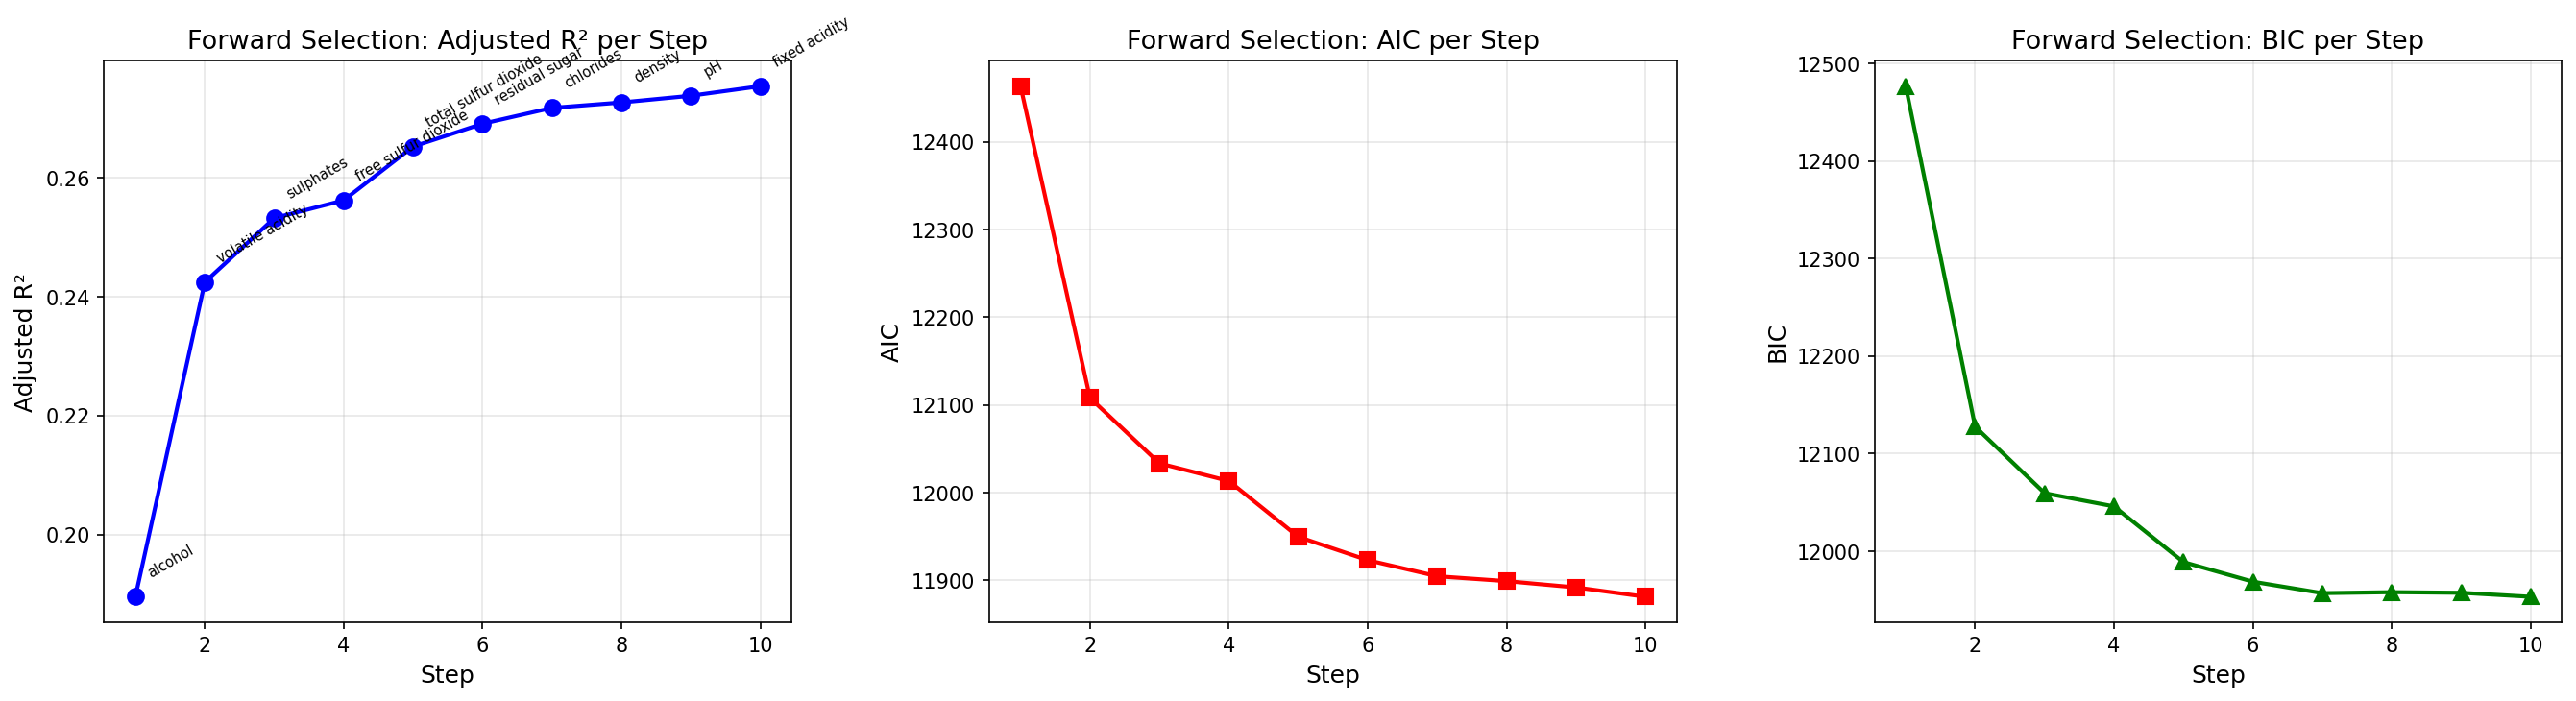
\includegraphics[width=\textwidth]{forward_selection_progression.png}
    \caption{Εξέλιξη των κριτηρίων $R^2_{adj}$, AIC και BIC κατά τα βήματα της πρόσω επιλογής. Παρατηρήστε ότι ο $R^2_{adj}$ αυξάνεται ολοένα και πιο αργά (φθίνουσα οριακή απόδοση), ενώ το AIC μειώνεται (βελτιώνεται) σε κάθε βήμα.}
    \label{fig:forward}
\end{figure}

\subsection{Ερμηνεία αποτελεσμάτων}

\subsubsection{Κεντρικά ευρήματα}

\begin{importantbox}[Κεντρικά ευρήματα πρόσω επιλογής]
\begin{enumerate}
    \item \textbf{Τελικό μοντέλο}: Περιλαμβάνει \textbf{10 από τις 11 μεταβλητές}. Αποκλείεται μόνο το \textbf{citric acid} ($p = 0.138 > 0.05$).

    \item \textbf{Ποιότητα προσαρμογής}: $R^2 = 0.2768$, $R^2_{adj} = 0.2755$. Δηλαδή το μοντέλο εξηγεί περίπου το 27.5\% της μεταβλητότητας -- ακριβώς όσο και το πλήρες μοντέλο του Υποερωτήματος 2, χωρίς τη μία <<περιττή>> μεταβλητή.

    \item \textbf{Ιεραρχία σπουδαιότητας}: Οι 3 πρώτες μεταβλητές (alcohol, volatile acidity, sulphates) εξηγούν ήδη $R^2_{adj} = 0.253$, δηλαδή \textbf{το 92\%} αυτού που εξηγεί το πλήρες μοντέλο.

    \item \textbf{Τα βήματα 4--10 προσθέτουν ελάχιστα}: Συνολικά $+0.022$ στον $R^2_{adj}$. Ένας αναλυτής θα μπορούσε εύλογα να κρατήσει μόνο τις 3 πρώτες μεταβλητές για ένα πιο <<φειδωλό>> μοντέλο.
\end{enumerate}
\end{importantbox}

\subsubsection{Γιατί η σειρά εισόδου διαφέρει από την απλή παλινδρόμηση;}

\begin{warningbox}[Η σειρά εισόδου αντικατοπτρίζει τη μοναδική συνεισφορά!]
Ένα ενδιαφέρον παράδειγμα: Στην απλή παλινδρόμηση (Υποερώτημα 1), η πυκνότητα (density) είχε πολύ χαμηλή p-value ($p < 10^{-100}$) και ήταν η δεύτερη πιο σημαντική μεταβλητή. Στη forward selection, μπαίνει μόλις στο \textbf{βήμα 8} (οκτώ!).

\textbf{Εξήγηση}: Η πυκνότητα εξαρτάται φυσικά από:
\begin{itemize}
    \item Το αλκοόλ (μπήκε στο βήμα 1) -- το αλκοόλ μειώνει την πυκνότητα
    \item Τα υπολειπόμενα σάκχαρα (βήμα 6) -- τα σάκχαρα αυξάνουν την πυκνότητα
\end{itemize}
Αφού αυτές οι μεταβλητές ήδη υπάρχουν στο μοντέλο, η πυκνότητα δεν <<μαθαίνει>> τίποτα νέο -- η πληροφορία της είναι ήδη <<καλυμμένη>>. Γι' αυτό η \textbf{μοναδική} της συνεισφορά είναι μικροσκοπική ($\Delta R^2_{adj} = +0.0009$).

Αντίθετα, τα sulphates μπαίνουν τρίτα γιατί δίνουν πληροφορία \textbf{εντελώς διαφορετική} από το alcohol και τη volatile acidity.
\end{warningbox}

\subsubsection{Σύγκριση με το πλήρες μοντέλο (Υποερώτημα 2)}

\begin{theorybox}[Πρόσω επιλογή vs Πλήρες μοντέλο]
\begin{center}
\begin{tabular}{lcc}
\toprule
\textbf{Χαρακτηριστικό} & \textbf{Πλήρες μοντέλο} & \textbf{Forward selection} \\
\midrule
Αριθμός μεταβλητών & 11 & 10 \\
$R^2_{adj}$ & 0.2757 & 0.2755 \\
Μη σημαντική μεταβλητή & citric acid ($p=0.138$) & citric acid (απορρίφθηκε) \\
\bottomrule
\end{tabular}
\end{center}

\textbf{Συμπέρασμα}: Τα δύο μοντέλα είναι \textbf{ουσιαστικά ισοδύναμα}! Η forward selection απλά επιβεβαιώνει ότι το citric acid δεν χρειάζεται -- αφαιρώντας το, χάνουμε μόλις $0.0002$ στον $R^2_{adj}$ (αμελητέα διαφορά).

Αυτή η συμφωνία μεταξύ δύο διαφορετικών μεθόδων (p-value ελέγχου στην πολλαπλή παλινδρόμηση + forward selection) \textbf{ενισχύει την εμπιστοσύνη μας} στο αποτέλεσμα.
\end{theorybox}

\subsubsection{Πρακτική σημασία: Αν είχαμε μόνο 3 μεταβλητές;}

\begin{examplebox}[Πρακτικό σενάριο: Ένα απλό μοντέλο για οινοποιεία]
Αν ένα μικρό οινοποιείο ήθελε ένα \textbf{απλό} και \textbf{πρακτικό} μοντέλο πρόβλεψης ποιότητας, θα μπορούσε να χρησιμοποιήσει μόνο τις 3 πρώτες μεταβλητές:
\begin{itemize}
    \item \textbf{Alcohol} (ποσοστό αλκοόλ)
    \item \textbf{Volatile acidity} (πτητική οξύτητα -- δείκτης <<ξυδιού>>)
    \item \textbf{Sulphates} (θειικά -- σχετίζονται με τη συντήρηση)
\end{itemize}

Αυτό το μοντέλο 3 μεταβλητών εξηγεί $R^2_{adj} = 0.253$, ενώ το πλήρες μοντέλο 10 μεταβλητών εξηγεί $R^2_{adj} = 0.2755$. Η διαφορά είναι μόλις $0.022$ (2.2 ποσοστιαίες μονάδες). Για πρακτικούς σκοπούς, αυτό μπορεί να αξίζει τον κόπο -- τρεις μετρήσεις αντί για δέκα!
\end{examplebox}

\textbf{Το τελικό μοντέλο πρόσω επιλογής:}
\begin{align*}
\text{quality} &= 43.86 + 0.274 \cdot \text{alcohol} - 1.300 \cdot \text{volatile\_acidity} \\
&+ 0.779 \cdot \text{sulphates} + 0.007 \cdot \text{free\_SO}_2 \\
&- 0.003 \cdot \text{total\_SO}_2 + 0.029 \cdot \text{residual\_sugar} \\
&- 1.267 \cdot \text{chlorides} - 42.70 \cdot \text{density} \\
&+ 0.394 \cdot \text{pH} + 0.047 \cdot \text{fixed\_acidity}
\end{align*}

\begin{theorybox}[Ανάγνωση του τελικού μοντέλου]
Πώς διαβάζουμε αυτήν την εξίσωση; Κάθε συντελεστής μας λέει \textbf{πόσο αλλάζει η ποιότητα} για κάθε μοναδιαία αύξηση της αντίστοιχης μεταβλητής, \textbf{κρατώντας όλες τις άλλες σταθερές}:
\begin{itemize}
    \item $+0.274 \cdot \text{alcohol}$: Κάθε 1\% αύξηση αλκοόλ $\to$ ποιότητα +0.274 βαθμούς
    \item $-1.300 \cdot \text{volatile acidity}$: Κάθε μονάδα αύξηση πτητικής οξύτητας $\to$ ποιότητα -1.300 βαθμούς (αρνητική επίδραση!)
    \item $-42.70 \cdot \text{density}$: Ο μεγάλος συντελεστής δεν σημαίνει μεγάλη επίδραση -- η πυκνότητα κυμαίνεται σε πολύ μικρό εύρος ($\approx 0.99$--$1.00$), άρα η πραγματική επίδραση είναι μικρή
\end{itemize}
\end{theorybox}


%==========================================================================
% ΥΠΟΕΡΩΤΗΜΑ 4: ΠΟΛΥΩΝΥΜΙΚΗ ΠΑΛΙΝΔΡΟΜΗΣΗ
%==========================================================================
\newpage
\section{Πολυωνυμική Παλινδρόμηση (Υποερώτημα 4)}

\subsection{Θεωρητικό υπόβαθρο}

\subsubsection{Πέρα από τη γραμμικότητα}

\begin{theorybox}[Ορισμός: Πολυωνυμική Παλινδρόμηση]
Μέχρι τώρα, υποθέταμε ότι η σχέση μεταξύ $X$ και $Y$ είναι \textbf{γραμμική} (ευθεία γραμμή). Αλλά στην πραγματικότητα, οι σχέσεις μπορεί να είναι \textbf{καμπυλωτές}. Η πολυωνυμική παλινδρόμηση επιτρέπει τη μοντελοποίηση τέτοιων σχέσεων:

\begin{equation}
Y = \beta_0 + \beta_1 X + \beta_2 X^2 + \beta_3 X^3 + \varepsilon
\end{equation}

\begin{itemize}
    \item \textbf{Γραμμικό μοντέλο} ($Y = \beta_0 + \beta_1 X$): Ευθεία γραμμή
    \item \textbf{Τετραγωνικό μοντέλο} ($Y = \beta_0 + \beta_1 X + \beta_2 X^2$): Παραβολή -- η σχέση μπορεί να αλλάξει κατεύθυνση μία φορά
    \item \textbf{Κυβικό μοντέλο} ($Y = \beta_0 + \beta_1 X + \beta_2 X^2 + \beta_3 X^3$): Η σχέση μπορεί να αλλάξει κατεύθυνση δύο φορές
\end{itemize}
\end{theorybox}

\begin{examplebox}[Γιατί χρειαζόμαστε πολυωνυμική παλινδρόμηση;]
Σκεφτείτε τη σχέση μεταξύ ποσότητας λιπάσματος και παραγωγής φυτών:
\begin{itemize}
    \item Λίγο λίπασμα $\Rightarrow$ μικρή παραγωγή (λείπει θρεπτική ουσία)
    \item Μέτριο λίπασμα $\Rightarrow$ μεγάλη παραγωγή (ιδανική ποσότητα)
    \item Πολύ λίπασμα $\Rightarrow$ μικρή παραγωγή (<<καίει>> τα φυτά!)
\end{itemize}
Αυτή η σχέση σχηματίζει μια \textbf{ανεστραμμένη παραβολή} ($\cap$) -- δεν μπορεί να αποτυπωθεί από ευθεία γραμμή!
\end{examplebox}

\subsubsection{Πώς ελέγχουμε τη μη γραμμικότητα;}

\begin{theorybox}[Έλεγχος μη γραμμικότητας]
Για να ελέγξουμε αν η σχέση είναι μη γραμμική, εφαρμόζουμε τον κυβικό μοντέλο και ελέγχουμε:
\begin{enumerate}
    \item Αν $\beta_3 \neq 0$ (σημαντικός κυβικός όρος) $\Rightarrow$ η σχέση είναι κυβική
    \item Αν $\beta_3 = 0$ αλλά $\beta_2 \neq 0$ (σημαντικός τετραγωνικός όρος) $\Rightarrow$ τετραγωνική σχέση
    \item Αν $\beta_3 = \beta_2 = 0$ $\Rightarrow$ η γραμμική σχέση αρκεί
\end{enumerate}

\textbf{Σημαντικό}: Παρόλο που τεχνικά προσθέτουμε $X^2$ και $X^3$, αυτό \textbf{παραμένει} γραμμική παλινδρόμηση ως προς τους \textbf{συντελεστές} $\beta$. Απλώς οι <<μεταβλητές>> μας τώρα είναι $X$, $X^2$ και $X^3$.
\end{theorybox}

\subsection{Αποτελέσματα}

Εξετάσαμε τις μεταβλητές \textbf{Residual Sugar}, \textbf{Chlorides} και \textbf{Alcohol}.

\subsubsection{Residual Sugar (Υπολειπόμενη ζάχαρη)}

\begin{table}[H]
\centering
\caption{Σύγκριση μοντέλων: quality $\sim$ residual sugar}
\begin{tabular}{lccccc}
\toprule
\textbf{Μοντέλο} & $R^2$ & $R^2_{adj}$ & \textbf{AIC} & \textbf{BIC} & \textbf{p-value ανώτερου όρου} \\
\midrule
Γραμμικό & 0.0029 & 0.0027 & 13557 & 13571 & -- \\
Τετραγωνικό & 0.0031 & 0.0027 & 13558 & 13578 & $0.297$ (NS) \\
Κυβικό & 0.0072 & 0.0066 & 13539 & 13565 & $2.99 \times 10^{-6}$ \\
\bottomrule
\end{tabular}
\end{table}

\textbf{Ανάλυση}: Ο τετραγωνικός όρος δεν είναι σημαντικός ($p = 0.297$), αλλά ο κυβικός είναι πολύ σημαντικός ($p = 2.99 \times 10^{-6}$). Αυτό σημαίνει ότι η σχέση μεταξύ ζάχαρης και ποιότητας είναι \textbf{μη γραμμική}. Ωστόσο, η βελτίωση σε $R^2$ είναι πολύ μικρή (από 0.0029 σε 0.0072), υποδεικνύοντας ότι η ζάχαρη παραμένει αδύναμος προβλέπτης.

\subsubsection{Chlorides (Χλωριούχα)}

\begin{table}[H]
\centering
\caption{Σύγκριση μοντέλων: quality $\sim$ chlorides}
\begin{tabular}{lccccc}
\toprule
\textbf{Μοντέλο} & $R^2$ & $R^2_{adj}$ & \textbf{AIC} & \textbf{BIC} & \textbf{p-value ανώτερου όρου} \\
\midrule
Γραμμικό & 0.0414 & 0.0412 & 13350 & 13363 & -- \\
Τετραγωνικό & 0.0583 & 0.0579 & 13258 & 13278 & $3.93 \times 10^{-22}$ \\
Κυβικό & 0.0708 & 0.0702 & 13190 & 13216 & $4.94 \times 10^{-17}$ \\
\bottomrule
\end{tabular}
\end{table}

\textbf{Ανάλυση}: Τόσο ο τετραγωνικός ($p = 3.93 \times 10^{-22}$) όσο και ο κυβικός όρος ($p = 4.94 \times 10^{-17}$) είναι εξαιρετικά σημαντικοί. Τα chlorides δείχνουν την \textbf{ισχυρότερη μη γραμμικότητα} από τις τρεις μεταβλητές. Η σχέση δεν είναι απλά <<όσο αυξάνονται τα χλωριούχα, μειώνεται η ποιότητα>> -- η μείωση επιταχύνεται σε υψηλές τιμές chlorides.

\subsubsection{Alcohol (Αλκοόλ)}

\begin{table}[H]
\centering
\caption{Σύγκριση μοντέλων: quality $\sim$ alcohol}
\begin{tabular}{lccccc}
\toprule
\textbf{Μοντέλο} & $R^2$ & $R^2_{adj}$ & \textbf{AIC} & \textbf{BIC} & \textbf{p-value ανώτερου όρου} \\
\midrule
Γραμμικό & 0.1897 & 0.1895 & 12463 & 12477 & -- \\
Τετραγωνικό & 0.1903 & 0.1900 & 12461 & 12481 & $0.046$ \\
Κυβικό & 0.1947 & 0.1943 & 12434 & 12461 & $6.56 \times 10^{-8}$ \\
\bottomrule
\end{tabular}
\end{table}

\textbf{Ανάλυση}: Ο τετραγωνικός όρος είναι οριακά σημαντικός ($p = 0.046$) και ο κυβικός πολύ σημαντικός ($p = 6.56 \times 10^{-8}$). Η σχέση αλκοόλ-ποιότητας δεν είναι τελείως γραμμική, αλλά η βελτίωση είναι μικρή ($R^2$: 0.190 $\rightarrow$ 0.195). Αυτό σημαίνει ότι η γραμμική προσέγγιση είναι <<αρκετά καλή>>, αν και τεχνικά η κυβική είναι καλύτερη.

\begin{figure}[H]
    \centering
    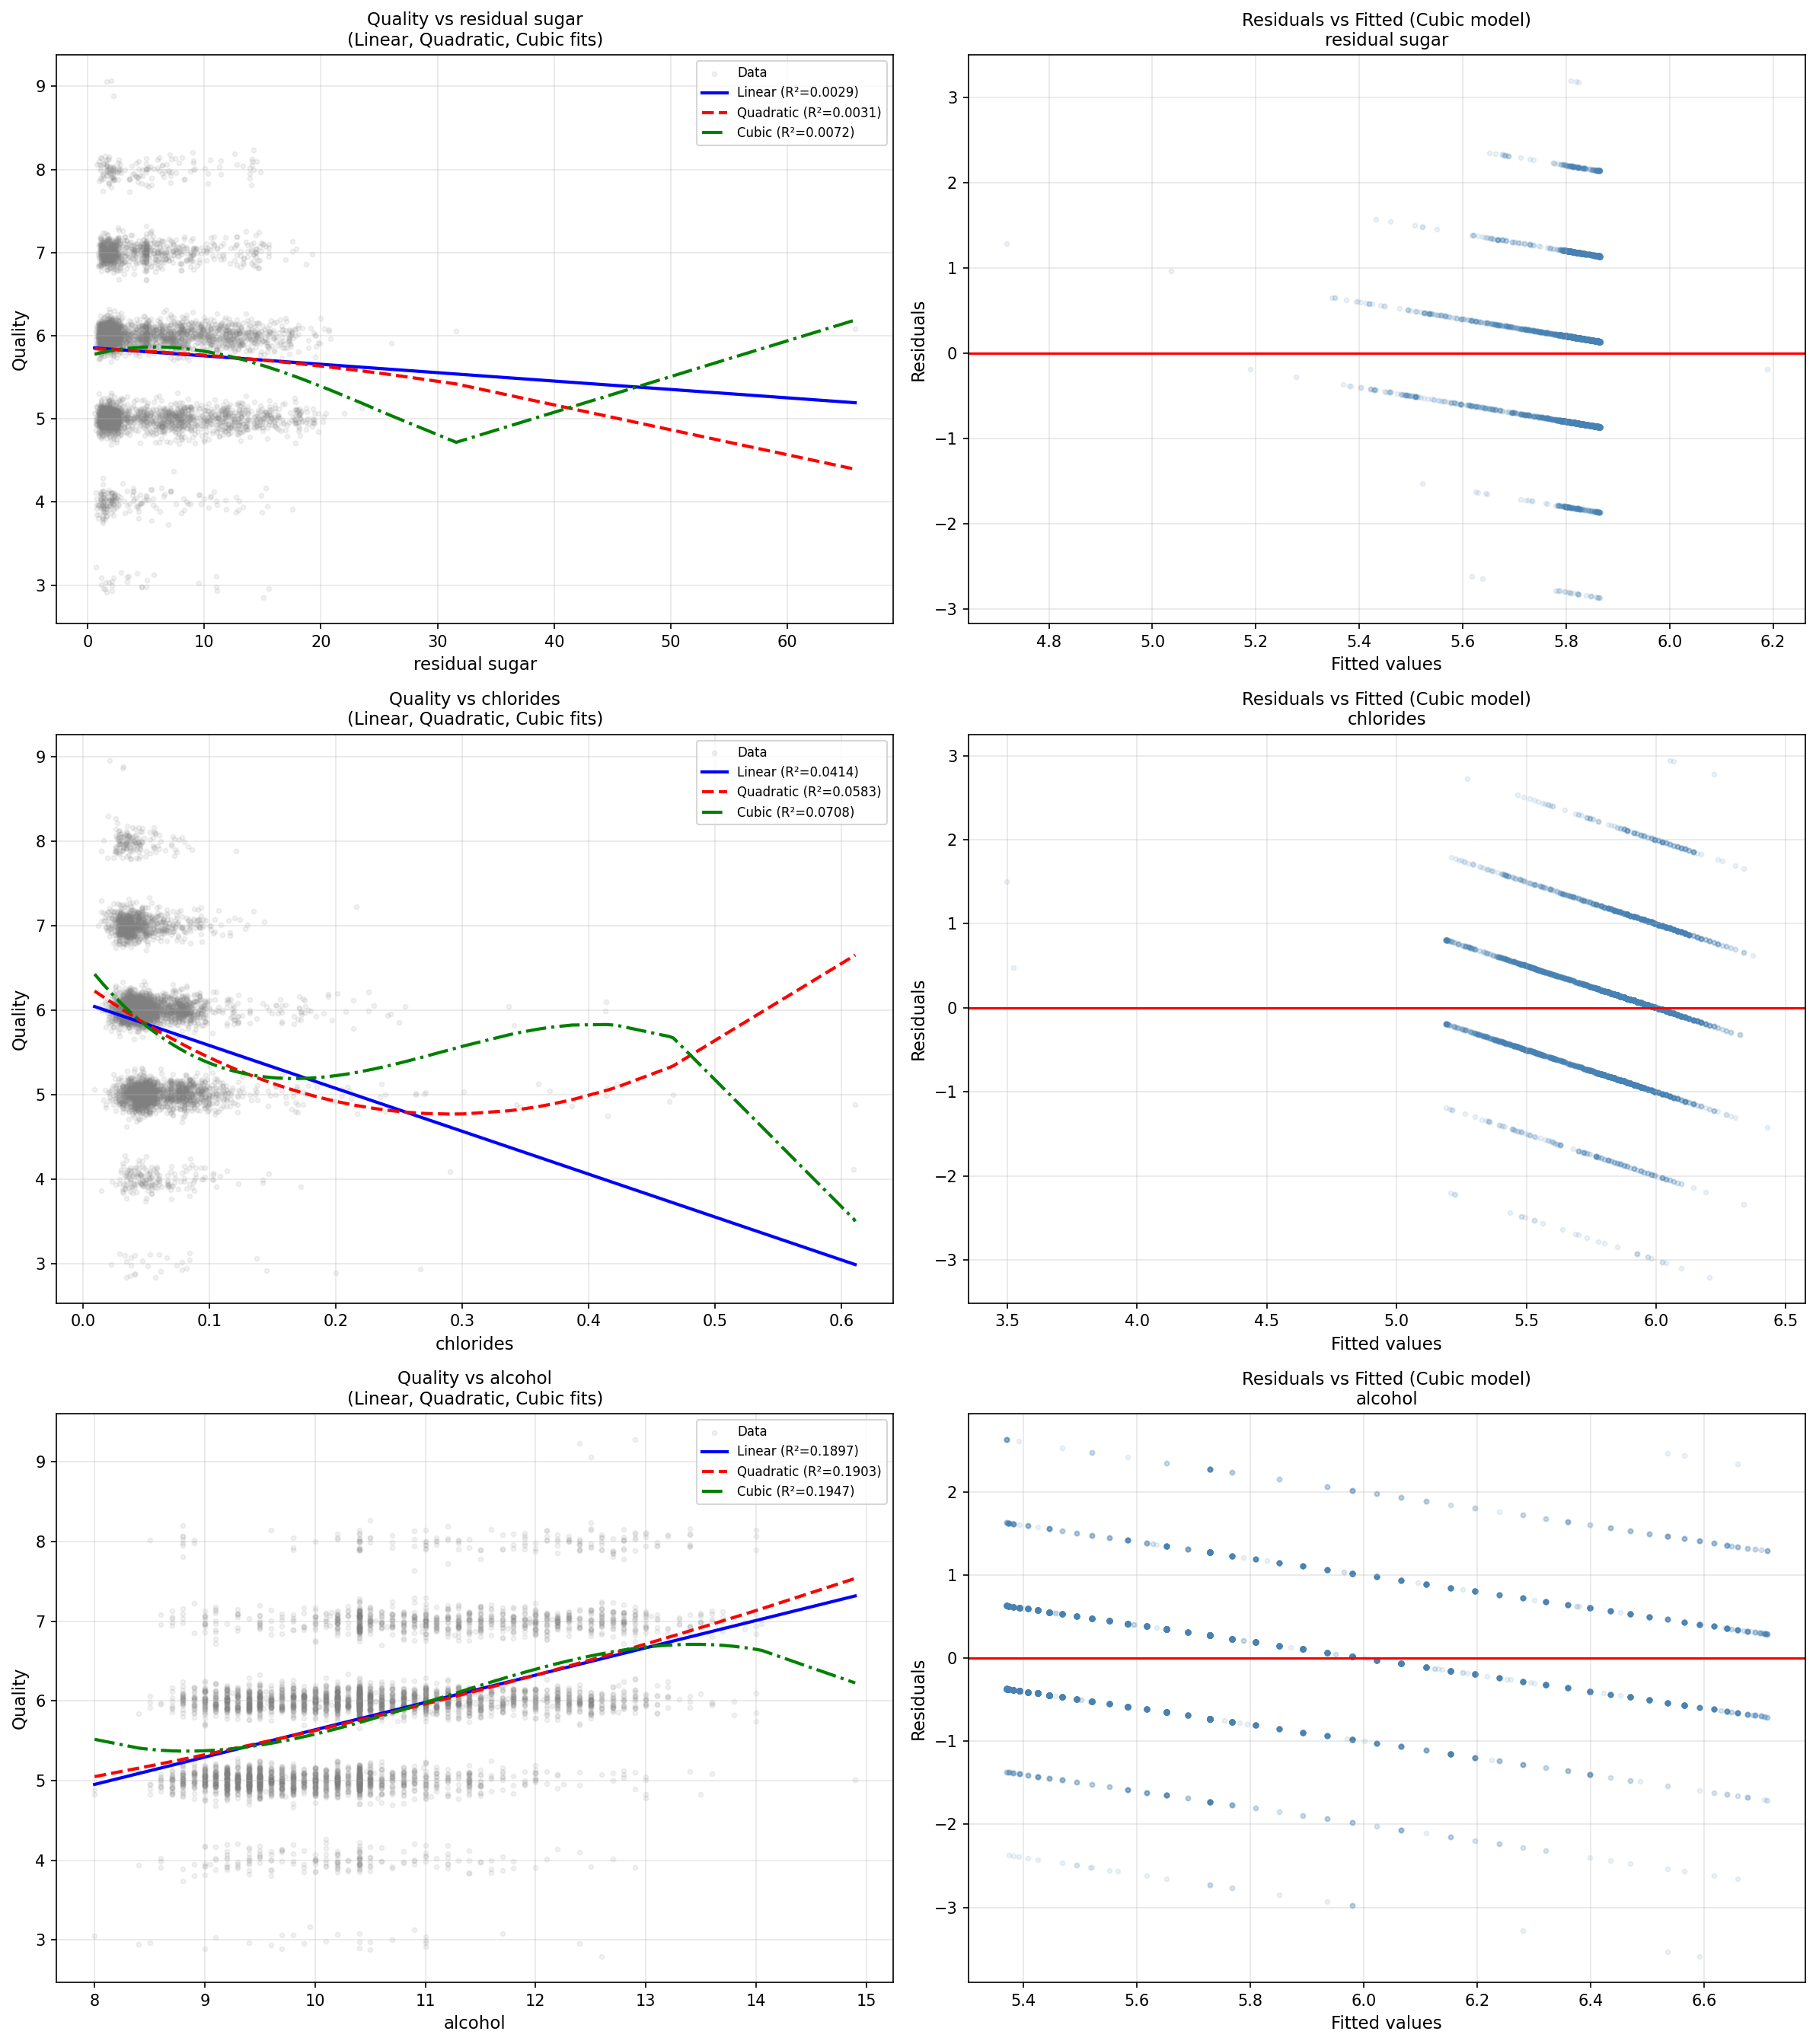
\includegraphics[width=\textwidth]{polynomial_regression.png}
    \caption{Πολυωνυμική παλινδρόμηση: Αριστερά τα scatter plots με τις τρεις καμπύλες προσαρμογής (γραμμική, τετραγωνική, κυβική). Δεξιά τα διαγράμματα υπολοίπων (residuals) για το βέλτιστο μοντέλο κάθε μεταβλητής.}
    \label{fig:polynomial}
\end{figure}

\subsubsection{Συνολική αξιολόγηση}

\begin{importantbox}[Συμπεράσματα πολυωνυμικής παλινδρόμησης]
\textbf{Και οι τρεις μεταβλητές δείχνουν ενδείξεις μη γραμμικής σχέσης} με την ποιότητα:
\begin{enumerate}
    \item \textbf{Chlorides}: Ισχυρή μη γραμμικότητα -- τόσο ο τετραγωνικός όσο και ο κυβικός όρος είναι πολύ σημαντικοί. Η σχέση είναι σαφώς κυβική.
    \item \textbf{Alcohol}: Σημαντικός κυβικός όρος, αλλά η πρακτική βελτίωση είναι μικρή.
    \item \textbf{Residual Sugar}: Σημαντικός κυβικός (αλλά όχι τετραγωνικός) όρος. Πολύ ασθενής σχέση συνολικά.
\end{enumerate}

\textbf{Σημαντική παρατήρηση}: Παρόλο που η μη γραμμικότητα είναι \textbf{στατιστικά σημαντική}, η \textbf{πρακτική βελτίωση} σε $R^2$ είναι μικρή. Αυτό σημαίνει ότι η αλλαγή μορφής (από γραμμικό σε κυβικό) δεν λύνει το πρόβλημα της χαμηλής ερμηνευτικής ικανότητας.
\end{importantbox}


%==========================================================================
% ΥΠΟΕΡΩΤΗΜΑ 5: ΚΡΙΤΙΚΗ ΑΞΙΟΛΟΓΗΣΗ
%==========================================================================
\newpage
\section{Κριτική Αξιολόγηση του Μοντέλου (Υποερώτημα 5)}

\subsection{Θεωρητικό υπόβαθρο: Υποθέσεις της γραμμικής παλινδρόμησης}

\begin{theorybox}[Οι 5 βασικές υποθέσεις]
Η γραμμική παλινδρόμηση βασίζεται σε 5 βασικές υποθέσεις. Αν κάποια παραβιάζεται, τα αποτελέσματά μας μπορεί να μην είναι αξιόπιστα:

\begin{enumerate}
    \item \textbf{Γραμμικότητα}: Η σχέση μεταξύ $X$ και $Y$ είναι γραμμική
    \item \textbf{Ανεξαρτησία}: Οι παρατηρήσεις είναι ανεξάρτητες μεταξύ τους
    \item \textbf{Ομοσκεδαστικότητα}: Η διακύμανση των σφαλμάτων $\varepsilon$ είναι σταθερή
    \item \textbf{Κανονικότητα}: Τα σφάλματα $\varepsilon$ ακολουθούν κανονική κατανομή
    \item \textbf{Μη πολυσυγγραμμικότητα}: Οι μεταβλητές $X$ δεν είναι υπερβολικά συσχετισμένες μεταξύ τους
\end{enumerate}
\end{theorybox}

\subsection{Διαγνωστικοί έλεγχοι}

\begin{figure}[H]
    \centering
    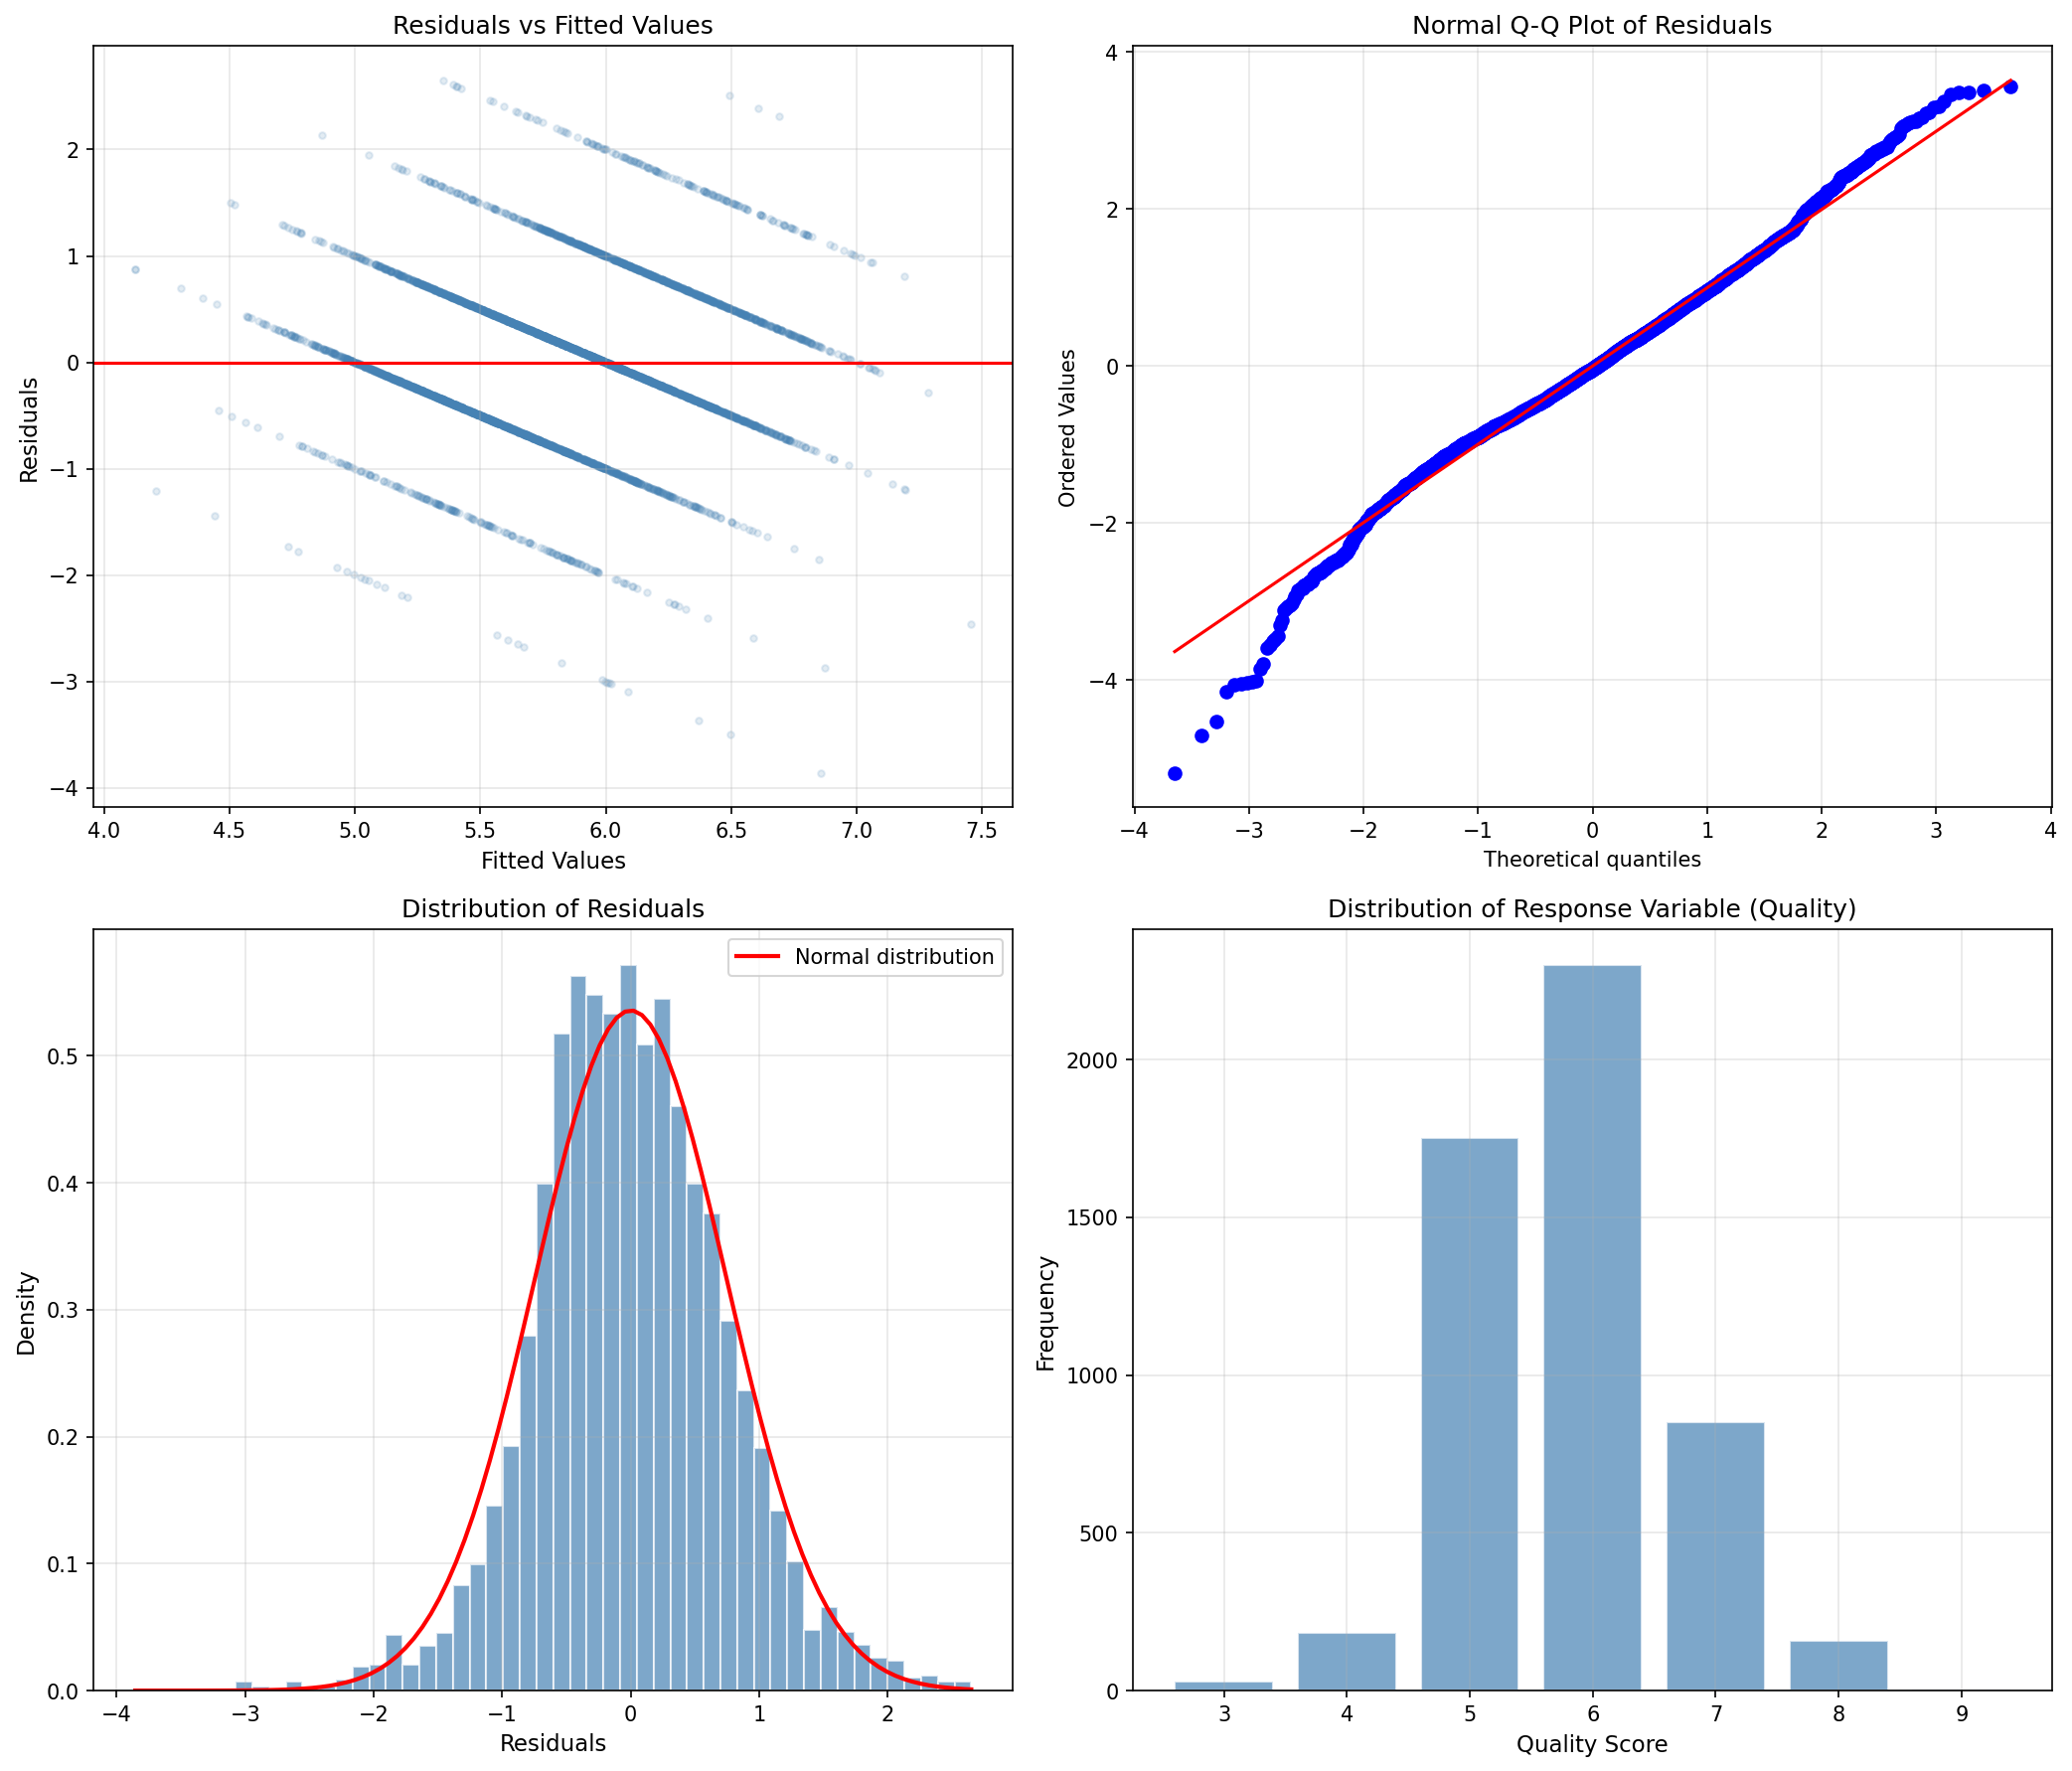
\includegraphics[width=\textwidth]{model_diagnostics.png}
    \caption{Διαγνωστικά γραφήματα: (a) Υπόλοιπα vs Προβλεπόμενες τιμές, (b) Q-Q plot κανονικότητας, (c) Κατανομή υπολοίπων, (d) Κατανομή μεταβλητής απόκρισης (quality).}
    \label{fig:diagnostics}
\end{figure}

\subsubsection{Έλεγχος 1: Κανονικότητα υπολοίπων}

\begin{theorybox}[Τι είναι τα υπόλοιπα (residuals);]
Τα \textbf{υπόλοιπα} είναι η διαφορά μεταξύ πραγματικής και προβλεπόμενης τιμής:
$$e_i = Y_i - \hat{Y}_i$$
Αν το μοντέλο λειτουργεί σωστά, τα υπόλοιπα πρέπει να μοιάζουν με \textbf{τυχαίο θόρυβο} -- δηλαδή να ακολουθούν κανονική κατανομή με μέσο 0.
\end{theorybox}

\textbf{Αποτελέσματα ελέγχων:}
\begin{itemize}
    \item \textbf{Shapiro-Wilk}: $W = 0.9912$, $p = 4.37 \times 10^{-17}$
    \item \textbf{Jarque-Bera}: $JB = 222.07$, $p = 5.99 \times 10^{-49}$
\end{itemize}

\begin{warningbox}[Πρόβλημα: Μη κανονικά υπόλοιπα]
Και οι δύο έλεγχοι \textbf{απορρίπτουν} την υπόθεση κανονικότητας ($p \ll 0.05$). Αυτό σημαίνει ότι τα confidence intervals και τα p-values μπορεί να μην είναι \textbf{ακριβή}.

Στο Q-Q plot (Σχήμα~\ref{fig:diagnostics}b) βλέπουμε αποκλίσεις στα \textbf{άκρα} (ουρές) -- τα ακραία υπόλοιπα είναι μεγαλύτερα από ό,τι θα περιμέναμε σε κανονική κατανομή.
\end{warningbox}

\subsubsection{Έλεγχος 2: Ομοσκεδαστικότητα}

\begin{theorybox}[Τι είναι η ομοσκεδαστικότητα;]
\textbf{Ομοσκεδαστικότητα} (homoscedasticity) σημαίνει ότι η <<διασπορά>> των σφαλμάτων είναι \textbf{ίδια} σε όλα τα επίπεδα πρόβλεψης. Αν η διασπορά αλλάζει (π.χ. μεγαλύτερη σε υψηλές τιμές), τότε έχουμε \textbf{ετεροσκεδαστικότητα} -- πρόβλημα!

\textbf{Οπτικός έλεγχος}: Στο γράφημα residuals vs fitted, τα σημεία πρέπει να σχηματίζουν μια <<λωρίδα>> σταθερού πλάτους. Αν η λωρίδα <<ανοίγει>> σαν χοάνη, υπάρχει ετεροσκεδαστικότητα.
\end{theorybox}

\textbf{Αποτέλεσμα Breusch-Pagan:} $BP = 75.01$, $p = 1.35 \times 10^{-11}$

\begin{warningbox}[Πρόβλημα: Ετεροσκεδαστικότητα]
Ο έλεγχος Breusch-Pagan απορρίπτει την ομοσκεδαστικότητα. Αυτό σημαίνει ότι τα \textbf{τυπικά σφάλματα} (standard errors) των συντελεστών μπορεί να μην είναι αξιόπιστα, και κατ' επέκταση τα t-tests και τα confidence intervals.
\end{warningbox}

\subsubsection{Έλεγχος 3: Αυτοσυσχέτιση}

\begin{theorybox}[Τι είναι η αυτοσυσχέτιση;]
Η \textbf{αυτοσυσχέτιση} (autocorrelation) σημαίνει ότι τα σφάλματα \textbf{διαδοχικών} παρατηρήσεων σχετίζονται μεταξύ τους. Ο έλεγχος \textbf{Durbin-Watson} ελέγχει αυτό, δίνοντας τιμή 0--4:
\begin{itemize}
    \item $DW \approx 2$: Δεν υπάρχει αυτοσυσχέτιση (ιδανικό)
    \item $DW \ll 2$: Θετική αυτοσυσχέτιση
    \item $DW \gg 2$: Αρνητική αυτοσυσχέτιση
\end{itemize}
\end{theorybox}

\textbf{Αποτέλεσμα}: $DW = 2.041 \approx 2$ -- \textbf{Δεν υπάρχει πρόβλημα αυτοσυσχέτισης.}

\subsubsection{Έλεγχος 4: Πολυσυγγραμμικότητα (VIF)}

\begin{theorybox}[Τι είναι η πολυσυγγραμμικότητα και ο VIF;]
Η \textbf{πολυσυγγραμμικότητα} (multicollinearity) υπάρχει όταν δύο ή περισσότερες προβλεπτικές μεταβλητές είναι ισχυρά συσχετισμένες μεταξύ τους. Αυτό δημιουργεί αστάθεια στις εκτιμήσεις των $\beta$.

Ο \textbf{VIF} (Variance Inflation Factor) μετράει πόσο <<φουσκωμένη>> είναι η διακύμανση ενός $\hat{\beta}_j$ λόγω συσχέτισης:
\begin{equation}
VIF_j = \frac{1}{1 - R_j^2}
\end{equation}
όπου $R_j^2$ είναι ο $R^2$ από την παλινδρόμηση του $X_j$ πάνω στα υπόλοιπα $X$.

\textbf{Εμπειρικοί κανόνες}:
\begin{itemize}
    \item $VIF < 5$: Αποδεκτό
    \item $5 < VIF < 10$: Μέτρια πολυσυγγραμμικότητα (πιθανό πρόβλημα)
    \item $VIF > 10$: Σοβαρή πολυσυγγραμμικότητα (σίγουρο πρόβλημα)
\end{itemize}
\end{theorybox}

\begin{table}[H]
\centering
\caption{Παράγοντας Πληθωρισμού Διακύμανσης (VIF) για κάθε μεταβλητή}
\label{tab:vif}
\begin{tabular}{lcc}
\toprule
\textbf{Μεταβλητή} & \textbf{VIF} & \textbf{Αξιολόγηση} \\
\midrule
\begin{english}fixed acidity\end{english} & 2.70 & Αποδεκτό \\
\begin{english}volatile acidity\end{english} & 1.85 & Αποδεκτό \\
\begin{english}citric acid\end{english} & 1.56 & Αποδεκτό \\
\begin{english}residual sugar\end{english} & 3.38 & Αποδεκτό \\
\begin{english}chlorides\end{english} & 1.59 & Αποδεκτό \\
\begin{english}free sulfur dioxide\end{english} & 2.09 & Αποδεκτό \\
\begin{english}total sulfur dioxide\end{english} & 2.79 & Αποδεκτό \\
\begin{english}density\end{english} & 6.26 & Μέτρια πολυσυγγρ. \\
\begin{english}pH\end{english} & 1.70 & Αποδεκτό \\
\begin{english}sulphates\end{english} & 1.41 & Αποδεκτό \\
\begin{english}alcohol\end{english} & 2.53 & Αποδεκτό \\
\bottomrule
\end{tabular}
\end{table}

\textbf{Ανάλυση}: Η πυκνότητα (density) εμφανίζει \textbf{μέτρια πολυσυγγραμμικότητα} ($VIF = 6.26$). Αυτό είναι φυσικό, καθώς η πυκνότητα εξαρτάται φυσικά από τη ζάχαρη και το αλκοόλ. Οι υπόλοιπες μεταβλητές δεν εμφανίζουν σημαντικό πρόβλημα.

\subsection{Κριτική αξιολόγηση: Είναι η παλινδρόμηση κατάλληλη;}

\begin{importantbox}[Βασικό πρόβλημα: Η μεταβλητή απόκρισης είναι διακριτή!]
Το \textbf{θεμελιώδες πρόβλημα} του μοντέλου μας είναι ότι η μεταβλητή quality δεν είναι συνεχής -- παίρνει ακέραιες τιμές (3, 4, 5, 6, 7, 8, 9). Η γραμμική παλινδρόμηση υποθέτει ότι η εξαρτημένη μεταβλητή είναι \textbf{συνεχής}.

Αυτό σημαίνει ότι:
\begin{itemize}
    \item Οι προβλέψεις μπορεί να πέφτουν \textbf{εκτός} του έγκυρου εύρους (π.χ. 4.7 ή 7.3 -- δεν υπάρχουν τέτοιοι βαθμοί)
    \item Τα υπόλοιπα εμφανίζουν χαρακτηριστικές \textbf{λωρίδες} (bands) αντί για ομοιογενή κατανομή
    \item Οι βασικές υποθέσεις κανονικότητας παραβιάζονται εξ αρχής
\end{itemize}
\end{importantbox}

\textbf{Σύνοψη όλων των προβλημάτων:}

\begin{enumerate}[label=\textbf{\arabic*.}]
    \item \textbf{Διακριτή μεταβλητή απόκρισης}: Η quality είναι τακτική (ordinal) με ακέραιες τιμές 3--9, ενώ η παλινδρόμηση υποθέτει συνεχή απόκριση.

    \item \textbf{Χαμηλή ερμηνευτική ικανότητα} ($R^2 \approx 27.7\%$): Το μοντέλο εξηγεί \textbf{λιγότερο από το ένα τρίτο} της μεταβλητότητας. Αυτό υποδεικνύει ότι:
    \begin{itemize}
        \item Υπάρχουν σημαντικοί παράγοντες που δεν περιλαμβάνονται στα δεδομένα
        \item Η ποιότητα κρασιού επηρεάζεται από υποκειμενικούς παράγοντες (π.χ. αξιολογητής, γεύση, αισθητική)
        \item Οι σχέσεις μπορεί να είναι πιο πολύπλοκες
    \end{itemize}

    \item \textbf{Μη κανονικά υπόλοιπα}: Οι έλεγχοι Shapiro-Wilk και Jarque-Bera απορρίπτουν σαφώς την κανονικότητα. Αυτό επηρεάζει τα confidence intervals και τα hypothesis tests.

    \item \textbf{Ετεροσκεδαστικότητα}: Ο έλεγχος Breusch-Pagan ($p = 1.35 \times 10^{-11}$) δείχνει ότι η διακύμανση των σφαλμάτων \textbf{δεν} είναι σταθερή, παραβιάζοντας μία ακόμη υπόθεση.

    \item \textbf{Πολυσυγγραμμικότητα}: Η πυκνότητα (density) εμφανίζει μέτρια πολυσυγγραμμικότητα ($VIF = 6.26$), καθώς εξαρτάται φυσικά από αλκοόλ και ζάχαρη.

    \item \textbf{Μη γραμμικές σχέσεις}: Όπως αποδείχθηκε στο Υποερώτημα 4, ορισμένες σχέσεις δεν είναι γραμμικές.
\end{enumerate}

\subsection{Εναλλακτικές προσεγγίσεις}

\begin{theorybox}[Τι θα μπορούσαμε να κάνουμε διαφορετικά;]
\begin{enumerate}
    \item \textbf{Τακτική λογιστική παλινδρόμηση} (Ordinal Logistic Regression): Σχεδιασμένη ειδικά για τακτικές εξαρτημένες μεταβλητές. Αντί να προβλέπει αριθμό, μοντελοποιεί τις \textbf{πιθανότητες} κάθε κατηγορίας.

    \item \textbf{Random Forest / Gradient Boosting}: Αλγόριθμοι μηχανικής μάθησης που:
    \begin{itemize}
        \item Δεν υποθέτουν γραμμικότητα
        \item Χειρίζονται αυτόματα αλληλεπιδράσεις μεταξύ μεταβλητών
        \item Συνήθως επιτυγχάνουν πολύ υψηλότερο $R^2$
    \end{itemize}

    \item \textbf{Ridge / LASSO παλινδρόμηση}: Παραλλαγές παλινδρόμησης που αντιμετωπίζουν την πολυσυγγραμμικότητα προσθέτοντας <<ποινή>> στους μεγάλους συντελεστές.

    \item \textbf{Παλινδρόμηση Poisson}: Κατάλληλη για μεταβλητές τύπου <<μέτρησης>> (count data), που μοιάζουν με τη quality.
\end{enumerate}
\end{theorybox}

%==========================================================================
% ΣΥΜΠΕΡΑΣΜΑΤΑ
%==========================================================================
\newpage
\section{Συμπεράσματα}

Η ανάλυση παλινδρόμησης στα δεδομένα ποιότητας κρασιού αποκάλυψε τα ακόλουθα:

\begin{enumerate}
    \item \textbf{Υποερώτημα 1 -- Απλή παλινδρόμηση}: Και οι 11 μεταβλητές εμφανίζουν στατιστικά σημαντικές σχέσεις με την ποιότητα. Ο ισχυρότερος μεμονωμένος προβλέπτης είναι το \textbf{αλκοόλ} ($R^2 = 0.19$), ακολουθούμενο από την πυκνότητα ($R^2 = 0.09$) και την πτητική οξύτητα ($R^2 = 0.06$).

    \item \textbf{Υποερώτημα 2 -- Πολλαπλή παλινδρόμηση}: Το πλήρες μοντέλο ($R^2 = 0.277$) εμφανίζει σημαντικούς συντελεστές για 10 από τις 11 μεταβλητές. Μοναδική εξαίρεση: το \textbf{citric acid} ($p = 0.138$), του οποίου η πληροφορία απορροφάται από τις υπόλοιπες μεταβλητές.

    \item \textbf{Υποερώτημα 3 -- Πρόσω επιλογή}: Η μέθοδος forward selection επέλεξε 10 μεταβλητές (εξαιρώντας πάλι το citric acid) με $R^2_{adj} = 0.2755$. Οι 3 πρώτες μεταβλητές (alcohol, volatile acidity, sulphates) παρέχουν ήδη τη μεγαλύτερη ερμηνευτική αξία.

    \item \textbf{Υποερώτημα 4 -- Πολυωνυμική παλινδρόμηση}: Υπάρχουν στατιστικά σημαντικές ενδείξεις μη γραμμικότητας και για τις τρεις μεταβλητές (residual sugar, chlorides, alcohol), με τα chlorides να εμφανίζουν την ισχυρότερη μη γραμμική σχέση.

    \item \textbf{Υποερώτημα 5 -- Κριτική}: Η γραμμική παλινδρόμηση δεν είναι η ιδανική επιλογή λόγω (α) διακριτής μεταβλητής απόκρισης, (β) χαμηλού $R^2$, (γ) παραβίασης υποθέσεων κανονικότητας και ομοσκεδαστικότητας. Εναλλακτικές όπως η τακτική λογιστική παλινδρόμηση ή αλγόριθμοι μηχανικής μάθησης θα ήταν πιο κατάλληλες.
\end{enumerate}

\vspace{1cm}

\begin{theorybox}[Τι μάθαμε;]
Η παλινδρόμηση είναι ένα \textbf{ισχυρό εργαλείο} αλλά όχι πανάκεια. Η σωστή χρήση της απαιτεί:
\begin{itemize}
    \item Κατανόηση των \textbf{υποθέσεών} της
    \item Κριτική σκέψη -- τα αποτελέσματα δεν αρκεί να είναι <<στατιστικά σημαντικά>>, πρέπει να είναι και \textbf{ουσιαστικά σημαντικά}
    \item Γνώση εναλλακτικών μεθόδων
    \item Διαγνωστικούς ελέγχους (residual analysis, VIF, κ.λπ.)
\end{itemize}

Σε αυτήν την εργασία, αν και η γραμμική παλινδρόμηση αποκάλυψε χρήσιμα μοτίβα (η σημασία του αλκοόλ, η αρνητική επίδραση της πτητικής οξύτητας), η χαμηλή ερμηνευτική ικανότητα ($R^2 \approx 28\%$) υπενθυμίζει ότι η ποιότητα κρασιού είναι ένα \textbf{πολύπλοκο} φαινόμενο που δεν μπορεί να αποδοθεί μόνο σε φυσικοχημικές ιδιότητες.
\end{theorybox}

\end{document}
